% Options for packages loaded elsewhere
\PassOptionsToPackage{unicode}{hyperref}
\PassOptionsToPackage{hyphens}{url}
%
\documentclass[
]{book}
\usepackage{amsmath,amssymb}
\usepackage{lmodern}
\usepackage{ifxetex,ifluatex}
\ifnum 0\ifxetex 1\fi\ifluatex 1\fi=0 % if pdftex
  \usepackage[T1]{fontenc}
  \usepackage[utf8]{inputenc}
  \usepackage{textcomp} % provide euro and other symbols
\else % if luatex or xetex
  \usepackage{unicode-math}
  \defaultfontfeatures{Scale=MatchLowercase}
  \defaultfontfeatures[\rmfamily]{Ligatures=TeX,Scale=1}
\fi
% Use upquote if available, for straight quotes in verbatim environments
\IfFileExists{upquote.sty}{\usepackage{upquote}}{}
\IfFileExists{microtype.sty}{% use microtype if available
  \usepackage[]{microtype}
  \UseMicrotypeSet[protrusion]{basicmath} % disable protrusion for tt fonts
}{}
\makeatletter
\@ifundefined{KOMAClassName}{% if non-KOMA class
  \IfFileExists{parskip.sty}{%
    \usepackage{parskip}
  }{% else
    \setlength{\parindent}{0pt}
    \setlength{\parskip}{6pt plus 2pt minus 1pt}}
}{% if KOMA class
  \KOMAoptions{parskip=half}}
\makeatother
\usepackage{xcolor}
\IfFileExists{xurl.sty}{\usepackage{xurl}}{} % add URL line breaks if available
\IfFileExists{bookmark.sty}{\usepackage{bookmark}}{\usepackage{hyperref}}
\hypersetup{
  pdftitle={S23 Summer School},
  pdfauthor={Caspar J. van Lissa¹ (only this GitBook; rest of the course by colleagues)},
  hidelinks,
  pdfcreator={LaTeX via pandoc}}
\urlstyle{same} % disable monospaced font for URLs
\usepackage{color}
\usepackage{fancyvrb}
\newcommand{\VerbBar}{|}
\newcommand{\VERB}{\Verb[commandchars=\\\{\}]}
\DefineVerbatimEnvironment{Highlighting}{Verbatim}{commandchars=\\\{\}}
% Add ',fontsize=\small' for more characters per line
\usepackage{framed}
\definecolor{shadecolor}{RGB}{248,248,248}
\newenvironment{Shaded}{\begin{snugshade}}{\end{snugshade}}
\newcommand{\AlertTok}[1]{\textcolor[rgb]{0.94,0.16,0.16}{#1}}
\newcommand{\AnnotationTok}[1]{\textcolor[rgb]{0.56,0.35,0.01}{\textbf{\textit{#1}}}}
\newcommand{\AttributeTok}[1]{\textcolor[rgb]{0.77,0.63,0.00}{#1}}
\newcommand{\BaseNTok}[1]{\textcolor[rgb]{0.00,0.00,0.81}{#1}}
\newcommand{\BuiltInTok}[1]{#1}
\newcommand{\CharTok}[1]{\textcolor[rgb]{0.31,0.60,0.02}{#1}}
\newcommand{\CommentTok}[1]{\textcolor[rgb]{0.56,0.35,0.01}{\textit{#1}}}
\newcommand{\CommentVarTok}[1]{\textcolor[rgb]{0.56,0.35,0.01}{\textbf{\textit{#1}}}}
\newcommand{\ConstantTok}[1]{\textcolor[rgb]{0.00,0.00,0.00}{#1}}
\newcommand{\ControlFlowTok}[1]{\textcolor[rgb]{0.13,0.29,0.53}{\textbf{#1}}}
\newcommand{\DataTypeTok}[1]{\textcolor[rgb]{0.13,0.29,0.53}{#1}}
\newcommand{\DecValTok}[1]{\textcolor[rgb]{0.00,0.00,0.81}{#1}}
\newcommand{\DocumentationTok}[1]{\textcolor[rgb]{0.56,0.35,0.01}{\textbf{\textit{#1}}}}
\newcommand{\ErrorTok}[1]{\textcolor[rgb]{0.64,0.00,0.00}{\textbf{#1}}}
\newcommand{\ExtensionTok}[1]{#1}
\newcommand{\FloatTok}[1]{\textcolor[rgb]{0.00,0.00,0.81}{#1}}
\newcommand{\FunctionTok}[1]{\textcolor[rgb]{0.00,0.00,0.00}{#1}}
\newcommand{\ImportTok}[1]{#1}
\newcommand{\InformationTok}[1]{\textcolor[rgb]{0.56,0.35,0.01}{\textbf{\textit{#1}}}}
\newcommand{\KeywordTok}[1]{\textcolor[rgb]{0.13,0.29,0.53}{\textbf{#1}}}
\newcommand{\NormalTok}[1]{#1}
\newcommand{\OperatorTok}[1]{\textcolor[rgb]{0.81,0.36,0.00}{\textbf{#1}}}
\newcommand{\OtherTok}[1]{\textcolor[rgb]{0.56,0.35,0.01}{#1}}
\newcommand{\PreprocessorTok}[1]{\textcolor[rgb]{0.56,0.35,0.01}{\textit{#1}}}
\newcommand{\RegionMarkerTok}[1]{#1}
\newcommand{\SpecialCharTok}[1]{\textcolor[rgb]{0.00,0.00,0.00}{#1}}
\newcommand{\SpecialStringTok}[1]{\textcolor[rgb]{0.31,0.60,0.02}{#1}}
\newcommand{\StringTok}[1]{\textcolor[rgb]{0.31,0.60,0.02}{#1}}
\newcommand{\VariableTok}[1]{\textcolor[rgb]{0.00,0.00,0.00}{#1}}
\newcommand{\VerbatimStringTok}[1]{\textcolor[rgb]{0.31,0.60,0.02}{#1}}
\newcommand{\WarningTok}[1]{\textcolor[rgb]{0.56,0.35,0.01}{\textbf{\textit{#1}}}}
\usepackage{longtable,booktabs,array}
\usepackage{calc} % for calculating minipage widths
% Correct order of tables after \paragraph or \subparagraph
\usepackage{etoolbox}
\makeatletter
\patchcmd\longtable{\par}{\if@noskipsec\mbox{}\fi\par}{}{}
\makeatother
% Allow footnotes in longtable head/foot
\IfFileExists{footnotehyper.sty}{\usepackage{footnotehyper}}{\usepackage{footnote}}
\makesavenoteenv{longtable}
\usepackage{graphicx}
\makeatletter
\def\maxwidth{\ifdim\Gin@nat@width>\linewidth\linewidth\else\Gin@nat@width\fi}
\def\maxheight{\ifdim\Gin@nat@height>\textheight\textheight\else\Gin@nat@height\fi}
\makeatother
% Scale images if necessary, so that they will not overflow the page
% margins by default, and it is still possible to overwrite the defaults
% using explicit options in \includegraphics[width, height, ...]{}
\setkeys{Gin}{width=\maxwidth,height=\maxheight,keepaspectratio}
% Set default figure placement to htbp
\makeatletter
\def\fps@figure{htbp}
\makeatother
\setlength{\emergencystretch}{3em} % prevent overfull lines
\providecommand{\tightlist}{%
  \setlength{\itemsep}{0pt}\setlength{\parskip}{0pt}}
\setcounter{secnumdepth}{5}
\usepackage{booktabs}
\usepackage{longtable}
\usepackage{array}
\usepackage{multirow}
\usepackage{wrapfig}
\usepackage{float}
\usepackage{colortbl}
\usepackage{pdflscape}
\usepackage{tabu}
\usepackage{threeparttable}
\usepackage{threeparttablex}
\usepackage[normalem]{ulem}
\usepackage{makecell}
\usepackage{xcolor}
\ifluatex
  \usepackage{selnolig}  % disable illegal ligatures
\fi

\title{S23 Summer School}
\usepackage{etoolbox}
\makeatletter
\providecommand{\subtitle}[1]{% add subtitle to \maketitle
  \apptocmd{\@title}{\par {\large #1 \par}}{}{}
}
\makeatother
\subtitle{Advanced Course on using Mplus}
\author{Caspar J. van Lissa¹ (only this GitBook; rest of the course by colleagues)}
\date{¹Utrecht University, Methodology \& Statistics}

\begin{document}
\maketitle

{
\setcounter{tocdepth}{1}
\tableofcontents
}
\hypertarget{course}{%
\chapter*{Course}\label{course}}
\addcontentsline{toc}{chapter}{Course}

This course material is part of the \href{https://utrechtsummerschool.nl/courses/social-sciences/advanced-course-on-using-mplus}{Advanced Course on using Mplus},
a five-day summer school course hosted by Utrecht University's department of Methodology and Statistics. If you already know how to analyse your data in Mplus but want to learn more about what you are actually doing, and especially if you want to know more about advanced longitudinal analyses, this course is for you. The course consists of in-depth lectures on the fundamentals of Mplus and advanced longitudinal models.

\hypertarget{preparing-for-the-course}{%
\chapter{Preparing for the course}\label{preparing-for-the-course}}

This Chapter helps you prepare for the course. It shows how to install R and RStudio on your computer. We'll also provide some general information on R, and how you can get help if you get error messages.

If you're already using R, all of this might be nothing new for you. You may \textbf{skip} this chapter then.

If you have \textbf{never used R before, this Chapter is essential}, as it gives you some input on how R works, and how we can use it for our data analyses.

\hypertarget{installing-software}{%
\section{Installing software}\label{installing-software}}

If you use R on your own computer, you will need to install it yourself. You should first:

\begin{enumerate}
\def\labelenumi{\arabic{enumi}.}
\tightlist
\item
  Install R from \url{https://CRAN.R-project.org}
\item
  Install `RStudio' Desktop (Free) from \url{https://rstudio.com}
\end{enumerate}

\begin{center}\rule{0.5\linewidth}{0.5pt}\end{center}

\hypertarget{installpackages}{%
\subsection{Installing packages}\label{installpackages}}

As a prerequisite for this guide, you need to have a few essential \textbf{R packages} installed.

\begin{enumerate}
\def\labelenumi{\arabic{enumi}.}
\tightlist
\item
  Open RStudio
\item
  Inside RStudio, find the window named \textbf{Console} on the bottom left corner of your screen (it might fill the entire left side of the screen).
\item
  We will now install a few packages using R Code. Here's an overview of the packages, and why we need them:
\end{enumerate}

\begin{tabular}{l|l}
\hline
Package & Description\\
\hline
MplusAutomation & Control Mplus from R and parse model output\\
\hline
ggplot2 & A flexible and user-friendly plotting package\\
\hline
tidySEM & Plotting and tabulating the output of SEM-models\\
\hline
semTools & Comparing models, establishing measurement invariance across groups\\
\hline
\end{tabular}

To install these packages, we use the \texttt{install.packages()} function in R. One package after another, our code should look like this:

\begin{Shaded}
\begin{Highlighting}[]
\FunctionTok{install.packages}\NormalTok{(}\StringTok{"MplusAutomation"}\NormalTok{)}
\FunctionTok{install.packages}\NormalTok{(}\StringTok{"ggplot2"}\NormalTok{)}
\FunctionTok{install.packages}\NormalTok{(}\StringTok{"tidySEM"}\NormalTok{)}
\FunctionTok{install.packages}\NormalTok{(}\StringTok{"semTools"}\NormalTok{)}
\end{Highlighting}
\end{Shaded}

\hypertarget{get-started}{%
\subsection{Get started}\label{get-started}}

\hypertarget{starting-a-new-project-in-rstudio}{%
\subsection{Starting a new project in Rstudio}\label{starting-a-new-project-in-rstudio}}

To keep all your work organized, you should use a \textbf{project}. In Rstudio, click on the \emph{New project} button:

\includegraphics{tut_new_proj.png}

In the pop-up dialog, click \emph{New directory}, and again \emph{New project}.

type the desired directory name in the dialog (give it a meaningful name, e.g.~``TCSM\_course''), and use `Browse' if you need to change the directory where you store your projects. Now, in your project, click \emph{File \textgreater{} New file \textgreater{} R script}. This script file works just like notepad, or the syntax editor in SPSS: You type plain text, but you can run it any time you want. Conduct all of the exercises in this script file.

\hypertarget{code-conventions}{%
\subsection{Code conventions}\label{code-conventions}}

Throughout the guide, a consistent set of conventions is used to refer to code:

\begin{itemize}
\tightlist
\item
  Functions are in a code font and followed by parentheses, like
  \texttt{sum()} or \texttt{mean()}.
\item
  Other R objects (like data or function arguments) are in a code
  font, without parentheses, like \texttt{seTE} or \texttt{method.tau}.
\item
  Sometimes, we'll use the package name followed by two colons, like
  \texttt{lavaan::sem()}. This is valid R code and will run. The \texttt{lavaan::} part indicates that the function \texttt{sem()} comes from the package \texttt{lavaan}.
\end{itemize}

\hypertarget{getting-help}{%
\subsection{Getting Help}\label{getting-help}}

As you start to apply the techniques described in this guide to your data you will soon find questions that the guide does not answer. This section describes a few tips on how to get help.

\begin{enumerate}
\def\labelenumi{\arabic{enumi}.}
\tightlist
\item
  Every function in R has documentation (a help file). To see it, select the name of the function and press F1, or run the command \texttt{?} followed by the name of the function, e.g.: \texttt{?aov}. I have been using R for 10 years, and I still press F1 all the time to see how a function works.
\item
  If you get stuck, start with \textbf{Google}. Typically, adding ``R'' to a search is enough to restrict it to relevant results, e.g.: ``exploratory factor analysis R.'' Google is particularly useful for error messages. If you get an error message and you have no idea what it means, try googling it. Chances are that someone else has been confused by it in the past, and there will be help somewhere on the web. (If the error message isn't in English,
  run \texttt{Sys.setenv(LANGUAGE\ =\ "en")} and re-run the code; you're
  more likely to find help for English error messages.)
\item
  If Google doesn't help, try \href{https://stackoverflow.com}{stackoverflow}. Start by spending a little time searching for an existing answer; including {[}R{]} restricts your search to questions and answers that use R.
\item
  Lastly, if you stumble upon an error (or typos!) in this guide's text or R syntax, feel free to contact \textbf{Caspar van Lissa} at \textbf{\href{mailto:c.j.vanlissa@uu.nl}{\nolinkurl{c.j.vanlissa@uu.nl}}}.
\end{enumerate}

\hypertarget{getting-the-course-data}{%
\section{Getting the course data}\label{getting-the-course-data}}

All of the course data files are available on a GitHub repository. You can download them all at once by going to \url{https://github.com/cjvanlissa/S23_student}, clicking the green button labeled `Code,' and downloading a ZIP archive of the repository.

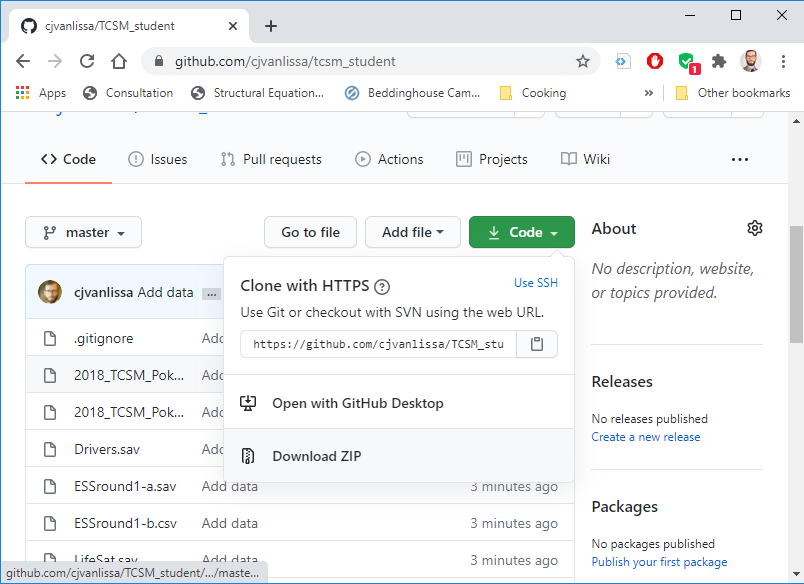
\includegraphics{coursematerials.png}

After unzipping the archive, you can open the RStudio project `S23\_student.Rproj,' and the script `run\_me.R.' This script contains a few lines of code to help you install the required R-packages for the course.

\hypertarget{r-tutorial-for-beginners-optional}{%
\section{R tutorial for beginners (optional)}\label{r-tutorial-for-beginners-optional}}

Welcome to the world of R! This tutorial is based on the tutorial ``R: How to get started'' by \href{https://www.linkedin.com/in/ihnwhi-heo/}{Ihnwhi Heo}, \href{https://www.ducoveen.com/}{Duco Veen}, and \href{https://www.rensvandeschoot.com/}{Rens van de Schoot}, and adapted for TCSM.

\hypertarget{who-r-you}{%
\subsection{Who R you?}\label{who-r-you}}

R is\ldots{}

\begin{itemize}
\tightlist
\item
  Free programming software for statistical computation and graphics
\item
  Open source: everyone (even you!) can improve, develop, and contribute to R
\item
  The official manual by the R Core Team: \href{https://cran.r-project.org/doc/manuals/r-release/R-intro.pdf}{An introduction to R}
\end{itemize}

R itself looks a bit old-fashioned and tedious:

\includegraphics{tut_R.jpg}

\hypertarget{rstudio}{%
\subsection{RStudio}\label{rstudio}}

Thankfully, we have a great user interface for R, called RStudio!

\begin{itemize}
\tightlist
\item
  RStudio helps users to use and learn R easier
\item
  If you are using RStudio, this means you are using R.
\item
  From now on, all tutorials will go with RStudio.
\end{itemize}

\hypertarget{no-pane-no-gain}{%
\subsubsection{No `pane,' no gain!}\label{no-pane-no-gain}}

When you open RStudio, the screen may look like this. You may notice that the screen is divided into A `panes' (a pane is a division of a window):

\includegraphics{tut_panes.jpg}

Before we explain these three panes - I want you to add the fourth one, which you will see if you open an R script. An R script is like a ``new document'' in Microsoft Word. When you open an R script, the fourth pane appears.

\hypertarget{create-a-new-r-script}{%
\subsubsection{Create a new R script}\label{create-a-new-r-script}}

Click the icon with a plus sign on the paper. Click the icon highlighted by the red square:

\includegraphics{tut_new_file.png}

When you click the icon, a new script appears in a fourth pane on the upper left side of the screen

\includegraphics{tut_panes2.jpg}

The four panes really help become organized. In RStudio, you can do everything all together on one screen. Thus, four panes make the work efficient (indeed, no `pain!').

\hypertarget{what-do-the-four-panes-do}{%
\subsubsection{What do the four panes do?}\label{what-do-the-four-panes-do}}

\begin{itemize}
\tightlist
\item
  Out of four panes, the two on the left side are the panes you will use a lot.

  \begin{itemize}
  \tightlist
  \item
    Source pane: located at the top left side of the screen. It is also called the ``editor,'' because this is where we edit scripts. We will usually type our code in the source pane.
  \item
    Console pane: located at the bottom left side of the screen. This panel is for direct communication with R. We can type commands here that are \emph{immediately} evaluated (whereas a script is only evaluated when we run it). Furthermore, all output of our commands is printed in this console pane.
  \end{itemize}
\item
  The panels on the right side of the screen contain various tabs. Among those tabs, it is worth looking at the Environment tab at the upper pane and the Plots tab at the lower pane.

  \begin{itemize}
  \tightlist
  \item
    The Environment tab contains all the `objects' currently loaded in your R session. In SPSS, you can have only one data file open. In R, you can have as many data `objects' as you like. They will be listed here. You can always check what objects are loaded under the environment tab. The environment is also called the `workspace.'
  \item
    The Plots tab shows various graphs and figures we draw. If you click Zoom with the magnifying glass, you can see plots in a bigger size.
  \end{itemize}
\end{itemize}

\hypertarget{day-2-latent-growth-models}{%
\chapter{Day 2: Latent Growth Models}\label{day-2-latent-growth-models}}

This computer lab session demonstrates to run latent growth models in batch, using the R-package \texttt{MplusAutomation}.
Note that, if you do not want to automate part of your workflow (like making plots and tables), you can also use Mplus exclusively.
All of the input files for the exercises described in this GitBook are provided with the course materials.

To get started with today's computer lab, first open the project file called ``S23.Rproj.'' It should load in the program ``RStudio.'' The bottom right panel has several tabs, including one called ``Files.'' Click on ``Files'' in this bottom right tab, and click the file ``growth\_exercises.R.''

\hypertarget{exercise-1-burn-survivors}{%
\section{Exercise 1: burn survivors}\label{exercise-1-burn-survivors}}

The file ``PTSD.dat'' contains another data set on burn survivors.
An incomplete, basic Mplus syntax can be found in the file
``PTSD - M0.inp.''

Specifying that same syntax could be done in R, using \texttt{MplusAutomation}, as well.
First, load the file \texttt{PTSD.dat} into the R environment.
For convenience's sake, rename the columns of the data object to something a human would understand:

\begin{Shaded}
\begin{Highlighting}[]
\NormalTok{data }\OtherTok{\textless{}{-}} \FunctionTok{read.table}\NormalTok{(}\StringTok{"PTSD.dat"}\NormalTok{, }\AttributeTok{na.strings =} \SpecialCharTok{{-}}\DecValTok{999}\NormalTok{)}
\FunctionTok{names}\NormalTok{(data) }\OtherTok{\textless{}{-}} \FunctionTok{c}\NormalTok{(}\StringTok{"gender"}\NormalTok{, }\StringTok{"tvlo"}\NormalTok{,}
                 \StringTok{"W1"}\NormalTok{, }\StringTok{"W2"}\NormalTok{, }\StringTok{"W3"}\NormalTok{, }\StringTok{"W4"}\NormalTok{, }\StringTok{"W5"}\NormalTok{, }\StringTok{"W6"}\NormalTok{, }\StringTok{"W7"}\NormalTok{, }\StringTok{"W8"}\NormalTok{,}
                 \StringTok{"pain"}\NormalTok{)}
\end{Highlighting}
\end{Shaded}

To specify a basic, \emph{incomplete} syntax, use:

\begin{Shaded}
\begin{Highlighting}[]
\NormalTok{basic }\OtherTok{\textless{}{-}} \FunctionTok{mplusObject}\NormalTok{(}
  \AttributeTok{TITLE =} \StringTok{"exercise 1"}\NormalTok{,}
  \AttributeTok{MODEL =} \StringTok{""}\NormalTok{,}
  \AttributeTok{OUTPUT =} \StringTok{"standardized;"}\NormalTok{,}
  \AttributeTok{PLOT =} \StringTok{"SERIES = w1{-}w8 (s);}
\StringTok{          TYPE = PLOT3;"}\NormalTok{,}
  \AttributeTok{rdata =}\NormalTok{ data,}
  \AttributeTok{usevariables =}
    \FunctionTok{c}\NormalTok{(}\StringTok{"W1"}\NormalTok{, }\StringTok{"W2"}\NormalTok{, }\StringTok{"W3"}\NormalTok{, }\StringTok{"W4"}\NormalTok{, }\StringTok{"W5"}\NormalTok{, }\StringTok{"W6"}\NormalTok{, }\StringTok{"W7"}\NormalTok{, }\StringTok{"W8"}\NormalTok{)}
\NormalTok{)}
\end{Highlighting}
\end{Shaded}

To evaluate this model, you can use:

\begin{Shaded}
\begin{Highlighting}[]
\NormalTok{result }\OtherTok{\textless{}{-}} \FunctionTok{mplusModeler}\NormalTok{(basic, }\AttributeTok{modelout =} \StringTok{"basic.inp"}\NormalTok{, }\AttributeTok{run =}\NormalTok{ 1L)}
\end{Highlighting}
\end{Shaded}

To summarize the results, you can use:

\begin{Shaded}
\begin{Highlighting}[]
\CommentTok{\# For one model}
\FunctionTok{SummaryTable}\NormalTok{(result)}
\CommentTok{\# For more models}
\FunctionTok{SummaryTable}\NormalTok{(}\FunctionTok{list}\NormalTok{(result1, result2))}
\end{Highlighting}
\end{Shaded}

\hypertarget{exercise-1a}{%
\subsection{Exercise 1a}\label{exercise-1a}}

Specify a latent growth model. Consider different specifications discussed in the lecture, and try to find the best specification.

Use only the time measurements, not including additional
predictor variables.\\
Think about:

\begin{itemize}
\tightlist
\item
  which metric of time to use (see the SPSS file form more information about the variables);
\item
  the shape of the function (linear or quadratic);
  and base your decision of the best model on:\\
\item
  model fit indices;
\item
  model comparison tools;
\item
  plots;
\item
  interpretation of the model parameters.
\end{itemize}

Click to show answers

Here is an example of how to approach the problem:

\begin{Shaded}
\begin{Highlighting}[]
\CommentTok{\# First, create a linear model from the basic one}
\NormalTok{linear }\OtherTok{\textless{}{-}}\NormalTok{ basic}
\NormalTok{linear}\SpecialCharTok{$}\NormalTok{MODEL }\OtherTok{\textless{}{-}}
  \StringTok{"i s | W1@0.5 W2@1 W3@2 W4@4 W5@6 W6@9 W7@12 W8@18;"}
\NormalTok{result\_linear }\OtherTok{\textless{}{-}} 
  \FunctionTok{mplusModeler}\NormalTok{(linear, }\AttributeTok{modelout =} \StringTok{"linear.inp"}\NormalTok{, }\AttributeTok{run =}\NormalTok{ 1L)}
\CommentTok{\# Then, a quadratic one}
\NormalTok{quad }\OtherTok{\textless{}{-}}\NormalTok{ basic}
\NormalTok{quad}\SpecialCharTok{$}\NormalTok{MODEL }\OtherTok{\textless{}{-}}
  \StringTok{"i s q | W1@0.5 W2@1 W3@2 W4@4 W5@6 W6@9 W7@12 W8@18;"}
\NormalTok{result\_quad }\OtherTok{\textless{}{-}}
  \FunctionTok{mplusModeler}\NormalTok{(quad, }\AttributeTok{modelout =} \StringTok{"quad.inp"}\NormalTok{, }\AttributeTok{run =}\NormalTok{ 1L)}
\CommentTok{\# Then, a quadratic one with fixed variance}
\NormalTok{quad0 }\OtherTok{\textless{}{-}}\NormalTok{ basic}
\NormalTok{quad0}\SpecialCharTok{$}\NormalTok{MODEL }\OtherTok{\textless{}{-}}
  \StringTok{"i s q | W1@0.5 W2@1 W3@2 W4@4 W5@6 W6@9 W7@12 W8@18;}
\StringTok{   q@0;"}
\NormalTok{result\_quad0 }\OtherTok{\textless{}{-}}
  \FunctionTok{mplusModeler}\NormalTok{(quad0, }\AttributeTok{modelout =} \StringTok{"quad0.inp"}\NormalTok{, }\AttributeTok{run =}\NormalTok{ 1L)}
\CommentTok{\# Combine them both in a list:}
\NormalTok{results }\OtherTok{\textless{}{-}} \FunctionTok{list}\NormalTok{(result\_linear, result\_quad, result\_quad0)}
\CommentTok{\# Compare the fit:}
\FunctionTok{SummaryTable}\NormalTok{(results,}
             \AttributeTok{keepCols =} \FunctionTok{c}\NormalTok{(}\StringTok{"Filename"}\NormalTok{, }\StringTok{"Parameters"}\NormalTok{,}
                          \StringTok{"AIC"}\NormalTok{, }\StringTok{"BIC"}\NormalTok{, }\StringTok{"RMSEA\_Estimate"}\NormalTok{,}
                          \StringTok{"CFI"}\NormalTok{, }\StringTok{"TLI"}\NormalTok{, }\StringTok{"SRMR"}\NormalTok{))}
\end{Highlighting}
\end{Shaded}

\begin{tabular}[t]{l|r|r|r|r|r|r|r}
\hline
Filename & Parameters & AIC & BIC & RMSEA\_Estimate & CFI & TLI & SRMR\\
\hline
quad0.out & 14 & 14037 & 14085 & 0.13 & 0.94 & 0.94 & 0.08\\
\hline
linear.out & 13 & 14051 & 14096 & 0.14 & 0.93 & 0.94 & 0.08\\
\hline
quad.out & NA & NA & NA & NA & NA & NA & NA\\
\hline
\end{tabular}

\hypertarget{exercise-1b-add-covariates}{%
\subsection{Exercise 1b: Add covariates}\label{exercise-1b-add-covariates}}

Using the best fitting LGM model found above, regress the growth parameters on TVLO and regress Pain
on the growth parameters (see example from slides).
Are there gender differences in the regression of the
growth parameters on TVLO and in the regression of Pain on the growth parameters?

Click to show answers

\begin{Shaded}
\begin{Highlighting}[]
\CommentTok{\# Assuming quad0 was the best, start with that}
\NormalTok{covs }\OtherTok{\textless{}{-}}\NormalTok{ quad0}
\CommentTok{\# Add to the existing model}
\NormalTok{covs}\SpecialCharTok{$}\NormalTok{MODEL }\OtherTok{\textless{}{-}} \FunctionTok{c}\NormalTok{(covs}\SpecialCharTok{$}\NormalTok{MODEL,}
                \StringTok{"}
\StringTok{                i s on TVLO;}
\StringTok{                pain on i s; }
\StringTok{                MODEL male:}
\StringTok{                i on TVLO (m1);}
\StringTok{                s on TVLO (m2);}
\StringTok{                pain on i (m3);}
\StringTok{                pain on s (m4);}
\StringTok{                MODEL female:}
\StringTok{                i on TVLO (f1);}
\StringTok{                s on TVLO (f2);}
\StringTok{                pain on i (f3);}
\StringTok{                pain on s (f4);"}\NormalTok{)}
\CommentTok{\# Add new usevariables:}
\NormalTok{covs}\SpecialCharTok{$}\NormalTok{usevariables }\OtherTok{\textless{}{-}} \FunctionTok{c}\NormalTok{(covs}\SpecialCharTok{$}\NormalTok{usevariables,}
                       \StringTok{"tvlo"}\NormalTok{, }\StringTok{"gender"}\NormalTok{, }\StringTok{"pain"}\NormalTok{)}
\NormalTok{covs}\SpecialCharTok{$}\NormalTok{rdata}
\CommentTok{\# Add grouping variable:}
\NormalTok{covs}\SpecialCharTok{$}\NormalTok{VARIABLE }\OtherTok{\textless{}{-}} \StringTok{"GROUPING IS gender (1 = male 2 = female);"}
\CommentTok{\# Add parameter tests}
\NormalTok{covs}\SpecialCharTok{$}\NormalTok{MODELTEST }\OtherTok{\textless{}{-}} \StringTok{"m3 = f3; m4 = f4;"}
                
\NormalTok{result\_covs }\OtherTok{\textless{}{-}} \FunctionTok{mplusModeler}\NormalTok{(covs,}
                            \AttributeTok{modelout =} \StringTok{"covs.inp"}\NormalTok{,}
                            \AttributeTok{run =}\NormalTok{ 1L)}
\CommentTok{\# Obtain the model summaries; you need the Wald test for}
\CommentTok{\# the parameter difference tests.}
\FunctionTok{get\_summaries}\NormalTok{(result\_covs)}
\end{Highlighting}
\end{Shaded}

\begin{verbatim}
##   Mplus.version       Title AnalysisType   DataType Estimator Observations
## 1           8.6  exercise 1      GENERAL INDIVIDUAL        ML          240
##   NGroups NDependentVars NIndependentVars NContinuousLatentVars Parameters
## 1       2              9                1                     3         38
##   ChiSqM_Value ChiSqM_DF ChiSqM_PValue ChiSqBaseline_Value ChiSqBaseline_DF
## 1          285        88             0                2316               90
##   ChiSqBaseline_PValue    LL UnrestrictedLL  CFI  TLI   AIC   BIC  aBIC
## 1                    0 -7959          -7817 0.91 0.91 15994 16127 16006
##   RMSEA_Estimate RMSEA_90CI_LB RMSEA_90CI_UB RMSEA_pLT05 WaldChiSq_Value
## 1           0.14          0.12          0.15           0             0.5
##   WaldChiSq_DF WaldChiSq_PValue  SRMR  AICC Filename
## 1            2             0.78 0.089 16009 covs.out
\end{verbatim}

\hypertarget{visualization}{%
\subsubsection{Visualization}\label{visualization}}

If you want to plot the model for these two groups,
you can use the SEM graphing package \texttt{tidySEM}.
This flexible package produces fully customizable plots based on the R graphing package \texttt{ggplot2} for Mplus (and \texttt{lavaan}) models.
If you want to make publication quality graphs, \href{https://cjvanlissa.github.io/tidySEM/articles/Plotting_graphs.html}{here is an online tutorial for graph customization}.
The script below demonstrates how to plot a model using \texttt{tidySEM}. Assuming that we only want to visualize the regression part of the model, you could specify:

\begin{Shaded}
\begin{Highlighting}[]
\FunctionTok{library}\NormalTok{(tidySEM)}
\FunctionTok{library}\NormalTok{(dplyr)}
\NormalTok{lo }\OtherTok{\textless{}{-}} \FunctionTok{get\_layout}\NormalTok{(}\StringTok{""}\NormalTok{,     }\StringTok{"I"}\NormalTok{,   }\StringTok{""}\NormalTok{,}
                 \StringTok{"TVLO"}\NormalTok{, }\StringTok{""}\NormalTok{,   }\StringTok{"PAIN"}\NormalTok{,}
                 \StringTok{""}\NormalTok{,     }\StringTok{"S"}\NormalTok{,   }\StringTok{""}\NormalTok{, }\AttributeTok{rows =} \DecValTok{3}\NormalTok{)}
\FunctionTok{graph\_sem}\NormalTok{(result\_covs, }\AttributeTok{layout =}\NormalTok{ lo)}
\end{Highlighting}
\end{Shaded}

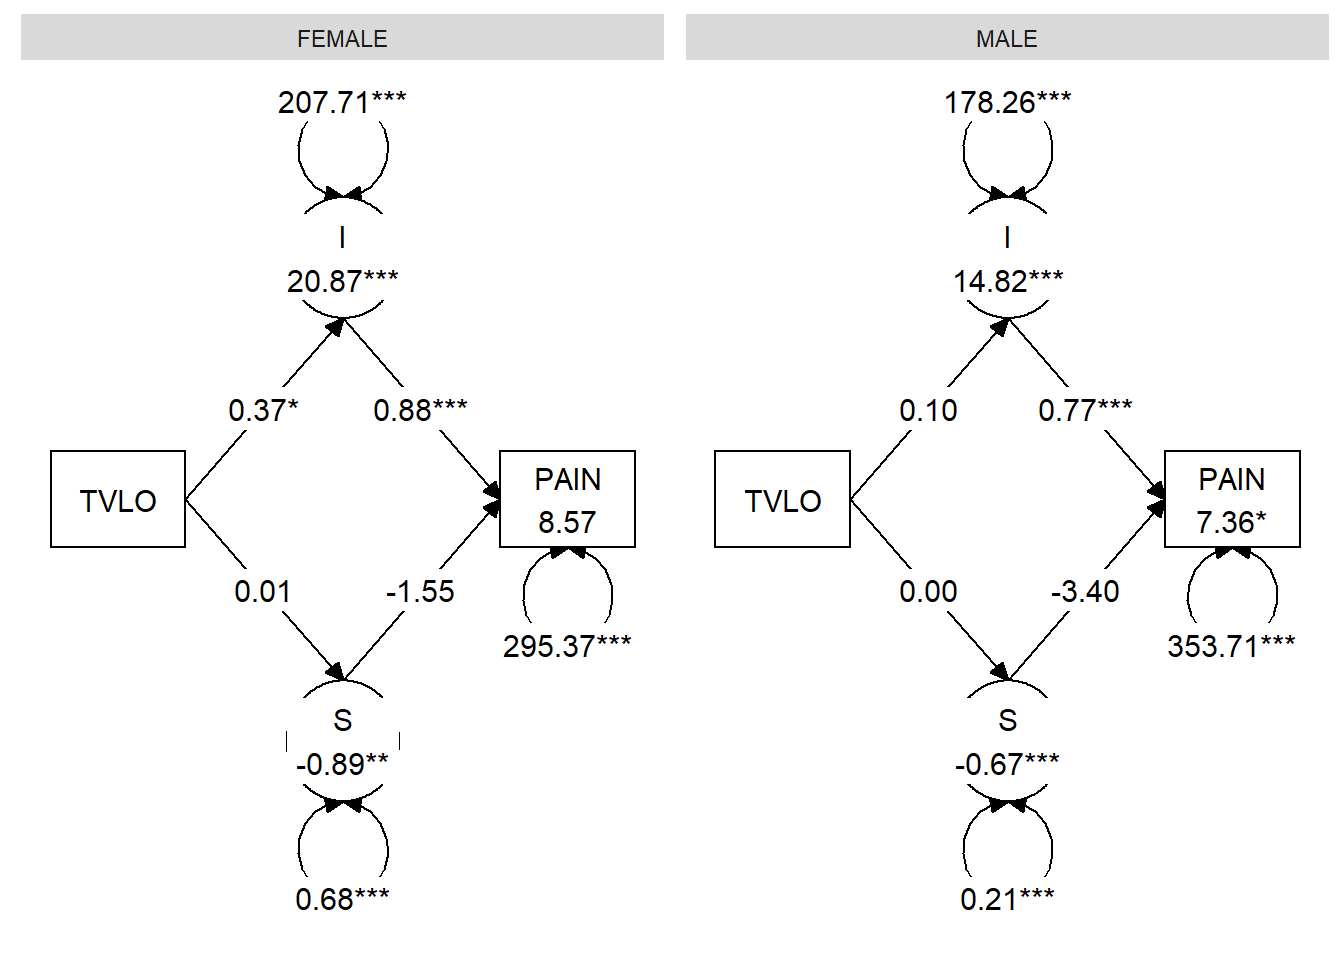
\includegraphics{S23_files/figure-latex/demotidysem1-1.pdf}

\hypertarget{tabulating-results}{%
\subsubsection{Tabulating results}\label{tabulating-results}}

In addition to graphing, it is also possible to tabulate the results using \texttt{tidySEM}.
Here is a brief example:

\begin{Shaded}
\begin{Highlighting}[]
\CommentTok{\# Get all columns of results}
\NormalTok{tab }\OtherTok{\textless{}{-}} \FunctionTok{table\_results}\NormalTok{(result\_covs, }\AttributeTok{columns =} \ConstantTok{NULL}\NormalTok{)}
\CommentTok{\# Retain regression parameters}
\NormalTok{tab }\OtherTok{\textless{}{-}}\NormalTok{ tab[tab}\SpecialCharTok{$}\NormalTok{op }\SpecialCharTok{==} \StringTok{"\textasciitilde{}"}\NormalTok{, ]}
\CommentTok{\# Remove group name from the label}
\NormalTok{tab}\SpecialCharTok{$}\NormalTok{label }\OtherTok{\textless{}{-}} \FunctionTok{gsub}\NormalTok{(}\StringTok{"}\SpecialCharTok{\textbackslash{}\textbackslash{}}\StringTok{.(FE)?MALE"}\NormalTok{, }\StringTok{""}\NormalTok{, tab}\SpecialCharTok{$}\NormalTok{label)}
\CommentTok{\# Make a wide table with both groups next to each other}
\NormalTok{tab }\OtherTok{\textless{}{-}} \FunctionTok{reshape}\NormalTok{(tab,}
               \AttributeTok{timevar =} \StringTok{"group"}\NormalTok{,}
               \AttributeTok{idvar =} \StringTok{"label"}\NormalTok{,}
               \AttributeTok{direction =} \StringTok{"wide"}\NormalTok{)}
\CommentTok{\# Retain only the standardized estimate, pvalue, and 95\% CI}
\NormalTok{tab[, }\FunctionTok{c}\NormalTok{(}\DecValTok{1}\NormalTok{, }\FunctionTok{grep}\NormalTok{(}\StringTok{"(est\_sig|pval|confint)\_std"}\NormalTok{, }\FunctionTok{names}\NormalTok{(tab)))]}
\end{Highlighting}
\end{Shaded}

\begin{tabular}[t]{l|l|l|l|l|l|l}
\hline
label & pval\_std.FEMALE & est\_sig\_std.FEMALE & confint\_std.FEMALE & pval\_std.MALE & est\_sig\_std.MALE & confint\_std.MALE\\
\hline
I.ON.TVLO & 0.01 & 0.31* & [ 0.06,  0.56] & 0.20 & 0.10 & [-0.05,  0.25]\\
\hline
PAIN.ON.I & 0.00 & 0.61*** & [ 0.43,  0.79] & 0.00 & 0.48*** & [ 0.36,  0.60]\\
\hline
PAIN.ON.S & 0.63 & -0.06 & [-0.31,  0.19] & 0.35 & -0.07 & [-0.22,  0.08]\\
\hline
S.ON.TVLO & 0.14 & 0.22 & [-0.07,  0.50] & 0.47 & 0.06 & [-0.11,  0.24]\\
\hline
\end{tabular}

\hypertarget{exercise-2-alcohol-use}{%
\section{Exercise 2: Alcohol use}\label{exercise-2-alcohol-use}}

The figure below depicts the basic Latent Growth model for the alcohol use data from Duncan, Duncan \& Strycker example 8\_1.

\begin{figure}
\centering
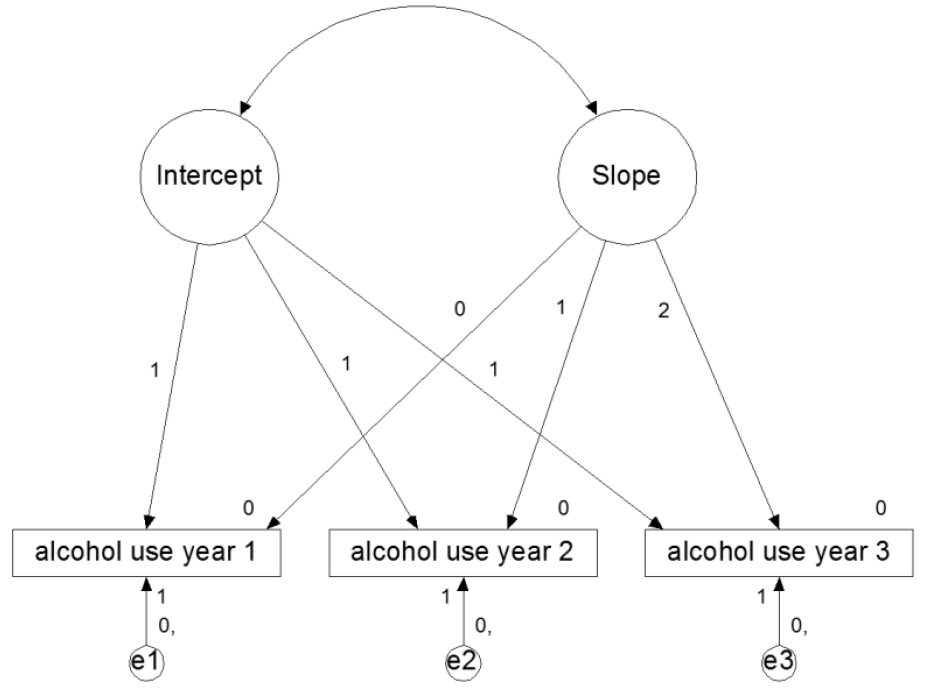
\includegraphics[width=4.16667in,height=\textheight]{./Materials/Figure1_lgm_alcohol.png}
\caption{Latent Growth model for alcohol}
\end{figure}

The data are in the file \texttt{DDS8\_1.dat}, with variables ALC1YR1 ALC1YR2 ALC1YR3 ALCPROB5 AGE1 and
GENDER1. Missing values are coded as -99. The variable ALCPROB5 is categorical, it indicates alcohol problems in
year 5 of the study (0=no, 1=yes).

First, load the file \texttt{DDS8\_1.dat} into the R environment. For convenience's sake, rename the columns of the data object to something a human would understand:

\begin{Shaded}
\begin{Highlighting}[]
\NormalTok{data }\OtherTok{\textless{}{-}} \FunctionTok{read.table}\NormalTok{(}\StringTok{"DDS8\_1.dat"}\NormalTok{, }\AttributeTok{na.strings =} \SpecialCharTok{{-}}\DecValTok{99}\NormalTok{)}
\FunctionTok{names}\NormalTok{(data) }\OtherTok{\textless{}{-}} \FunctionTok{c}\NormalTok{(}\StringTok{"ALC1YR1"}\NormalTok{, }\StringTok{"ALC1YR2"}\NormalTok{, }\StringTok{"ALC1YR3"}\NormalTok{,}
                 \StringTok{"ALCPROB5"}\NormalTok{, }\StringTok{"AGE1"}\NormalTok{, }\StringTok{"GENDER1"}\NormalTok{)}
\end{Highlighting}
\end{Shaded}

\hypertarget{exercise-2a}{%
\subsection{Exercise 2a}\label{exercise-2a}}

Set up the growth curve model as depicted in the Figure in Mplus.
As a starting point, use the \texttt{MplusAutomation} code below.

\begin{itemize}
\tightlist
\item
  Add the necessary syntax statements to finalize the syntax.
\item
  Request sample statistics and standardized (STDYX) output.
\item
  Inspect the output carefully with special attention for

  \begin{enumerate}
  \def\labelenumi{\arabic{enumi}.}
  \tightlist
  \item
    the pattern of missing values
  \item
    how well the model fits
  \item
    interpretation of the output; how well does the model predict alcohol use over the
    years?
  \end{enumerate}
\end{itemize}

\begin{Shaded}
\begin{Highlighting}[]
\NormalTok{m0 }\OtherTok{\textless{}{-}} \FunctionTok{mplusObject}\NormalTok{(}
  \AttributeTok{TITLE =} \StringTok{"LGA MODEL"}\NormalTok{,}
  \AttributeTok{MODEL =} \StringTok{""}\NormalTok{,}
  \AttributeTok{OUTPUT =} \StringTok{""}\NormalTok{,}
  \AttributeTok{rdata =}\NormalTok{ data,}
  \AttributeTok{usevariables =} \FunctionTok{c}\NormalTok{(}\StringTok{"ALC1YR1"}\NormalTok{, }\StringTok{"ALC1YR2"}\NormalTok{, }\StringTok{"ALC1YR3"}\NormalTok{))}
\end{Highlighting}
\end{Shaded}

Click to show answers

Here is an example of how to approach the problem:

\begin{Shaded}
\begin{Highlighting}[]
\NormalTok{m0 }\OtherTok{\textless{}{-}} \FunctionTok{mplusObject}\NormalTok{(}
  \AttributeTok{TITLE =} \StringTok{"LGA MODEL"}\NormalTok{,}
  \AttributeTok{MODEL =} \StringTok{"i s | ALC1YR1@0 ALC1YR2@1 ALC1YR3@2;"}\NormalTok{,}
  \AttributeTok{OUTPUT =} \StringTok{"SAMPSTAT standardized;"}\NormalTok{,}
  \AttributeTok{PLOT =} \StringTok{"SERIES = ALC1YR1 ALC1YR2 ALC1YR3 (s);}
\StringTok{            TYPE = PLOT3;"}\NormalTok{,}
  \AttributeTok{rdata =}\NormalTok{ data,}
  \AttributeTok{usevariables =} \FunctionTok{c}\NormalTok{(}\StringTok{"ALC1YR1"}\NormalTok{, }\StringTok{"ALC1YR2"}\NormalTok{, }\StringTok{"ALC1YR3"}\NormalTok{))}
\end{Highlighting}
\end{Shaded}

\hypertarget{exercise-2b}{%
\subsection{Exercise 2b}\label{exercise-2b}}

We will now \emph{explore} how different predictor variables affect the model fit.
Include gender and age in the model as predictors of the intercept and slope. Interpret the fit of the model
and the output.
Feel free to estimate several models, including or excluding certain covariates.
Either make a model fit table by hand in a spreadsheet, or use \texttt{SummaryTable()} to request the fit indices you deem to be appropriate.
Which model do you consider to be best?

\hypertarget{exploratory-vs-confirmatory-research}{%
\subsubsection{Exploratory vs confirmatory research}\label{exploratory-vs-confirmatory-research}}

Note that when you conduct \emph{confirmatory} research, and are testing theoretical hypotheses, you should not add and omit paths based on exploratory analyses and model fit.

It is fine to add and remove paths in \emph{exploratory} research. Model fit indices, like AIC and BIC, are suitable for selecting well-fitting models in exploratory research. P-values are not designed for variable selection, and using them for that purpose may lead to suboptimal models.

It is good scientific practice to clearly separate confirmatory and exploratory research. When you conduct exploratory research, you should not perform inference on the resulting parameters based on p-values (because inference generalizes your findings to the population, and exploratory findings tend to be tailored toward this specific sample).
You should also not present exploratory results as if they were testing a post-hoc theory (``Hypothesizing After the Results are Known,'' or HARKing, is a questionable research practice and can lead to false-positive (spurious) findings.

Click to show answers

The answers to Exercise 1a demonstrate how to approach this.
Estimate multiple slightly different models, put them in a list, and run \texttt{SummaryTable()}.
Then use the AIC and BIC to identify the best-fitting model,
and assess how different the model fits are.
Also consider using RMSEA, CFI, TLI, and SRMR to make sure that your best-fitting
model has acceptable objective fit.

\begin{Shaded}
\begin{Highlighting}[]
\CommentTok{\# Create a vector with three "additional syntaxes"}
\CommentTok{\# for my three different models}
\NormalTok{mod }\OtherTok{=} \FunctionTok{c}\NormalTok{(}\StringTok{"i s ON GENDER1;"}\NormalTok{,}
        \StringTok{"i s ON AGE1;"}\NormalTok{,}
        \StringTok{"i s ON AGE1 GENDER1;"}\NormalTok{,}
        \StringTok{"i ON GENDER1;"}\NormalTok{,}
        \StringTok{"i ON AGE1;"}\NormalTok{,}
        \StringTok{"i ON AGE1 GENDER1;"}\NormalTok{,}
        \StringTok{"s ON GENDER1;"}\NormalTok{,}
        \StringTok{"s ON AGE1;"}\NormalTok{,}
        \StringTok{"s ON AGE1 GENDER1;"}\NormalTok{,}
        \StringTok{"i WITH s@0;"}\NormalTok{,}
        \StringTok{"!baseline"}\NormalTok{)}
\CommentTok{\# Create a list with the additional usevariables}
\CommentTok{\# used in the three models above}
\NormalTok{vars }\OtherTok{=} \FunctionTok{list}\NormalTok{(}\StringTok{"GENDER1"}\NormalTok{,}
            \StringTok{"AGE1"}\NormalTok{,}
            \FunctionTok{c}\NormalTok{(}\StringTok{"GENDER1"}\NormalTok{, }\StringTok{"AGE1"}\NormalTok{),}
            \StringTok{"GENDER1"}\NormalTok{,}
            \StringTok{"AGE1"}\NormalTok{,}
            \FunctionTok{c}\NormalTok{(}\StringTok{"GENDER1"}\NormalTok{, }\StringTok{"AGE1"}\NormalTok{),}
            \StringTok{"GENDER1"}\NormalTok{,}
            \StringTok{"AGE1"}\NormalTok{,}
            \FunctionTok{c}\NormalTok{(}\StringTok{"GENDER1"}\NormalTok{, }\StringTok{"AGE1"}\NormalTok{),}
            \ConstantTok{NULL}\NormalTok{,}
            \ConstantTok{NULL}\NormalTok{)}
\CommentTok{\# Make a list of exploratory models by modifying m0}
\NormalTok{models }\OtherTok{\textless{}{-}} \FunctionTok{lapply}\NormalTok{(}\DecValTok{1}\SpecialCharTok{:}\FunctionTok{length}\NormalTok{(mod), }\ControlFlowTok{function}\NormalTok{(i)\{}
  \CommentTok{\# append element i of mod}
\NormalTok{  m0}\SpecialCharTok{$}\NormalTok{MODEL }\OtherTok{\textless{}{-}} \FunctionTok{paste0}\NormalTok{(m0}\SpecialCharTok{$}\NormalTok{MODEL, mod[i]) }
  \CommentTok{\# append element i of vars}
\NormalTok{  m0}\SpecialCharTok{$}\NormalTok{usevariables }\OtherTok{\textless{}{-}} \FunctionTok{c}\NormalTok{(m0}\SpecialCharTok{$}\NormalTok{usevariables, vars[[i]])}
  \CommentTok{\# Add unique filename}
\NormalTok{  m0}\SpecialCharTok{$}\NormalTok{modelout }\OtherTok{=} \FunctionTok{paste0}\NormalTok{(}\StringTok{"Model"}\NormalTok{, i, }\StringTok{".inp"}\NormalTok{) }
  \CommentTok{\# return the modified model}
\NormalTok{  m0 }
\NormalTok{\})}
\CommentTok{\# Run all models and store results in a list called results}
\NormalTok{results }\OtherTok{\textless{}{-}} \FunctionTok{lapply}\NormalTok{(models, mplusModeler, }\AttributeTok{run =}\NormalTok{ 1L)}
\CommentTok{\# Get summary table and store it in \textquotesingle{}tab\textquotesingle{}}
\NormalTok{tab }\OtherTok{\textless{}{-}} \FunctionTok{SummaryTable}\NormalTok{(results, }
                    \AttributeTok{keepCols =} \FunctionTok{c}\NormalTok{(}\StringTok{"Parameters"}\NormalTok{, }\StringTok{"AIC"}\NormalTok{, }\StringTok{"BIC"}\NormalTok{,}
                                 \StringTok{"RMSEA\_Estimate"}\NormalTok{, }\StringTok{"CFI"}\NormalTok{,}
                                 \StringTok{"TLI"}\NormalTok{, }\StringTok{"SRMR"}\NormalTok{),}
                    \AttributeTok{sortBy =} \ConstantTok{NULL}\NormalTok{)}
\CommentTok{\# Order by BIC}
\NormalTok{tab }\OtherTok{\textless{}{-}}\NormalTok{ tab[}\FunctionTok{order}\NormalTok{(tab}\SpecialCharTok{$}\NormalTok{BIC), ]}
\CommentTok{\# Add model syntax to the table}
\NormalTok{tab }\OtherTok{\textless{}{-}} \FunctionTok{cbind}\NormalTok{(}\AttributeTok{Model =}\NormalTok{ mod, tab)}
\NormalTok{tab}
\end{Highlighting}
\end{Shaded}

\begin{tabular}[t]{l|r|r|r|r|r|r|r}
\hline
Model & Parameters & AIC & BIC & RMSEA\_Estimate & CFI & TLI & SRMR\\
\hline
i s ON GENDER1; & 12 & 5129 & 5178 & 0.03 & 0.99 & 0.98 & 0.02\\
\hline
i s ON AGE1; & 10 & 5140 & 5181 & 0.03 & 1.00 & 0.98 & 0.02\\
\hline
i s ON AGE1 GENDER1; & 9 & 5166 & 5204 & 0.12 & 0.81 & 0.71 & 0.07\\
\hline
i ON GENDER1; & 8 & 5176 & 5209 & 0.06 & 0.99 & 0.97 & 0.02\\
\hline
i ON AGE1; & 10 & 5168 & 5209 & 0.05 & 0.99 & 0.96 & 0.02\\
\hline
i ON AGE1 GENDER1; & 8 & 5179 & 5212 & 0.15 & 0.80 & 0.69 & 0.08\\
\hline
s ON GENDER1; & 9 & 5199 & 5237 & 0.16 & 0.66 & 0.48 & 0.10\\
\hline
s ON AGE1; & 8 & 5207 & 5240 & 0.15 & 0.76 & 0.63 & 0.08\\
\hline
s ON AGE1 GENDER1; & 8 & 5208 & 5241 & 0.20 & 0.66 & 0.48 & 0.11\\
\hline
i WITH s@0; & 8 & 5211 & 5244 & 0.16 & 0.74 & 0.60 & 0.08\\
\hline
!baseline & 7 & 5217 & 5246 & 0.22 & 0.74 & 0.61 & 0.09\\
\hline
\end{tabular}

\begin{Shaded}
\begin{Highlighting}[]
\CommentTok{\# Plot the BICs and annotate with the syntax to see which is best}
\FunctionTok{library}\NormalTok{(ggplot2)}
\FunctionTok{qplot}\NormalTok{(}\AttributeTok{x =} \DecValTok{1}\SpecialCharTok{:}\DecValTok{11}\NormalTok{, }\AttributeTok{y =}\NormalTok{ tab}\SpecialCharTok{$}\NormalTok{BIC) }\SpecialCharTok{+}
  \FunctionTok{geom\_line}\NormalTok{() }\SpecialCharTok{+}
  \FunctionTok{geom\_text}\NormalTok{(}\AttributeTok{label =}\NormalTok{ tab}\SpecialCharTok{$}\NormalTok{Model, }\AttributeTok{size =} \DecValTok{2}\NormalTok{)}
\end{Highlighting}
\end{Shaded}

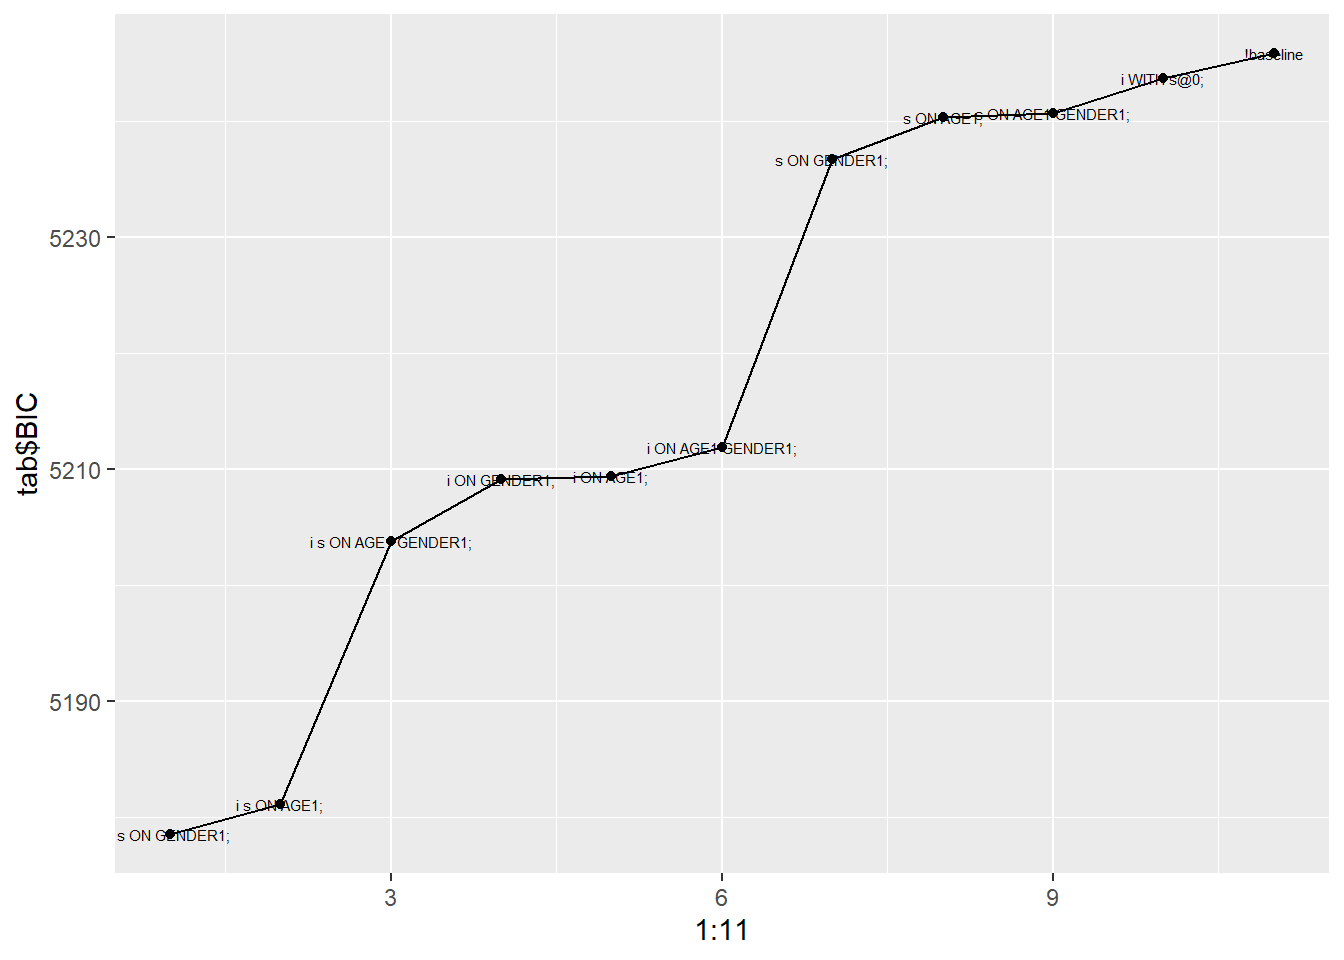
\includegraphics{S23_files/figure-latex/unnamed-chunk-16-1.pdf}

It looks like, paradoxically, predicting I and S from either age or gender
has the best fit. However, note that there is only a small difference between
the smallest and the largest BIC: diff(range(tab\$BIC)).
I would either go for the simplest model (i WITH \href{mailto:s@0}{\nolinkurl{s@0}}), or go for the
best-fitting model (i s ON GENDER1).

\hypertarget{exercise-2c}{%
\subsection{Exercise 2c}\label{exercise-2c}}

Include alcohol problems in year 5 in the model: let the intercept and slope factors predict alcohol problems year 5. Declare the variable as categorical in the variable section (CATEGORICAL = ALCPROB5).
Inspect if the effect of age and gender on alcohol problems year 5 is completely mediated by the growth
factors, or if there are additional direct paths from age and gender on the alcohol problems.

Click to show answers

To test whether there is full mediation or not, we want to test whether the direct
effects are equal to zero or not.

If the analysis had not included a categorical dependent variable,
then we would have been able to compute the difference test using MplusAutomation's
function \texttt{compareModels(model1,\ model2,\ diffTest\ =\ TRUE)}.

However, in the presence of a categorical dependent variable, we must use Mplus'
option \texttt{difftest}.

Again, we can start from m0:

\begin{Shaded}
\begin{Highlighting}[]
\CommentTok{\# Specify model with only indirect effects}
\NormalTok{m2c\_indirect }\OtherTok{\textless{}{-}}\NormalTok{ m0}
\NormalTok{m2c\_indirect}\SpecialCharTok{$}\NormalTok{usevariables }\OtherTok{\textless{}{-}} \FunctionTok{c}\NormalTok{(}
\NormalTok{  m2c\_indirect}\SpecialCharTok{$}\NormalTok{usevariables,}
  \StringTok{"AGE1"}\NormalTok{, }\StringTok{"GENDER1"}\NormalTok{, }\StringTok{"ALCPROB5"}\NormalTok{)}
\NormalTok{m2c\_indirect}\SpecialCharTok{$}\NormalTok{VARIABLE }\OtherTok{\textless{}{-}} \StringTok{"CATEGORICAL = ALCPROB5;"}
\NormalTok{m2c\_indirect}\SpecialCharTok{$}\NormalTok{MODEL }\OtherTok{\textless{}{-}} \FunctionTok{paste0}\NormalTok{(}
\NormalTok{  m0}\SpecialCharTok{$}\NormalTok{MODEL,}
  \StringTok{"i on AGE1 GENDER1;}
\StringTok{  i WITH s;}
\StringTok{  ALCPROB5 on i s;}
\StringTok{  ALCPROB5 on AGE1 GENDER1;"}\NormalTok{)}
\NormalTok{m2c\_indirect}\SpecialCharTok{$}\NormalTok{SAVEDATA }\OtherTok{\textless{}{-}} \StringTok{"difftest is mediation.dat;"}
\NormalTok{m2c\_indirect}\SpecialCharTok{$}\NormalTok{modelout }\OtherTok{\textless{}{-}} \StringTok{"m2c\_indirect.inp"}
\CommentTok{\# Run all models and store results in a list called results}
\NormalTok{result\_ind }\OtherTok{\textless{}{-}} \FunctionTok{mplusModeler}\NormalTok{(m2c\_indirect, }\AttributeTok{run =}\NormalTok{ 1L)}

\CommentTok{\# Specify model with direct effects too}
\NormalTok{m2c\_direct }\OtherTok{\textless{}{-}}\NormalTok{ m2c\_indirect}
\CommentTok{\# Constrain direct effects to 0 using gsub (replace)}
\NormalTok{m2c\_direct}\SpecialCharTok{$}\NormalTok{MODEL }\OtherTok{\textless{}{-}} \FunctionTok{gsub}\NormalTok{(}\StringTok{"ALCPROB5 on AGE1 GENDER1;"}\NormalTok{,}
                         \StringTok{"ALCPROB5 on AGE1 GENDER1@0;"}\NormalTok{,}
\NormalTok{                         m2c\_direct}\SpecialCharTok{$}\NormalTok{MODEL,}
                         \AttributeTok{fixed =} \ConstantTok{TRUE}\NormalTok{)}
\NormalTok{m2c\_direct}\SpecialCharTok{$}\NormalTok{ANALYSIS }\OtherTok{\textless{}{-}} \StringTok{"difftest = mediation.dat;"} 
\NormalTok{m2c\_direct}\SpecialCharTok{$}\NormalTok{modelout }\OtherTok{\textless{}{-}} \StringTok{"m2c\_direct.inp"}
\CommentTok{\# Run the direct model, which includes the difference test}
\NormalTok{result\_dir }\OtherTok{\textless{}{-}} \FunctionTok{mplusModeler}\NormalTok{(m2c\_direct, }\AttributeTok{run =}\NormalTok{ 1L)}
\CommentTok{\# Look at the model summaries}
\FunctionTok{get\_summaries}\NormalTok{(result\_dir)}
\end{Highlighting}
\end{Shaded}

\begin{verbatim}
##   Mplus.version      Title AnalysisType   DataType Estimator Observations
## 1           8.6  LGA MODEL      GENERAL INDIVIDUAL     WLSMV          466
##   NGroups NDependentVars NIndependentVars NContinuousLatentVars Parameters
## 1       1              4                2                     2         14
##   ChiSqM_Value ChiSqM_DF ChiSqM_PValue ChiSqBaseline_Value ChiSqBaseline_DF
## 1          5.1         7          0.64                 215               14
##   ChiSqBaseline_PValue ChiSqDiffTest_Value ChiSqDiffTest_DF
## 1                    0                0.21                1
##   ChiSqDiffTest_PValue CFI TLI RMSEA_Estimate RMSEA_90CI_LB RMSEA_90CI_UB
## 1                 0.64   1   1              0             0         0.047
##   RMSEA_pLT05  SRMR       Filename
## 1        0.96 0.057 m2c_direct.out
\end{verbatim}

Note that the ChiSqDiffTest\_PValue is non-significant, which means we can
prefer the simpler (no direct effects) model. There is full mediation.

Let's use a graph to examine the unconstrained model too:

\begin{Shaded}
\begin{Highlighting}[]
\NormalTok{lo }\OtherTok{\textless{}{-}} \FunctionTok{get\_layout}\NormalTok{(}\StringTok{"AGE1"}\NormalTok{,    }\StringTok{""}\NormalTok{, }\StringTok{""}\NormalTok{,}
                 \StringTok{""}\NormalTok{,        }\StringTok{"I"}\NormalTok{,  }\StringTok{"ALCPROB5"}\NormalTok{,}
                 \StringTok{"GENDER1"}\NormalTok{, }\StringTok{""}\NormalTok{, }\StringTok{""}\NormalTok{, }\AttributeTok{rows =} \DecValTok{3}\NormalTok{)}
\FunctionTok{graph\_sem}\NormalTok{(result\_ind, }\AttributeTok{layout =}\NormalTok{ lo)}
\end{Highlighting}
\end{Shaded}

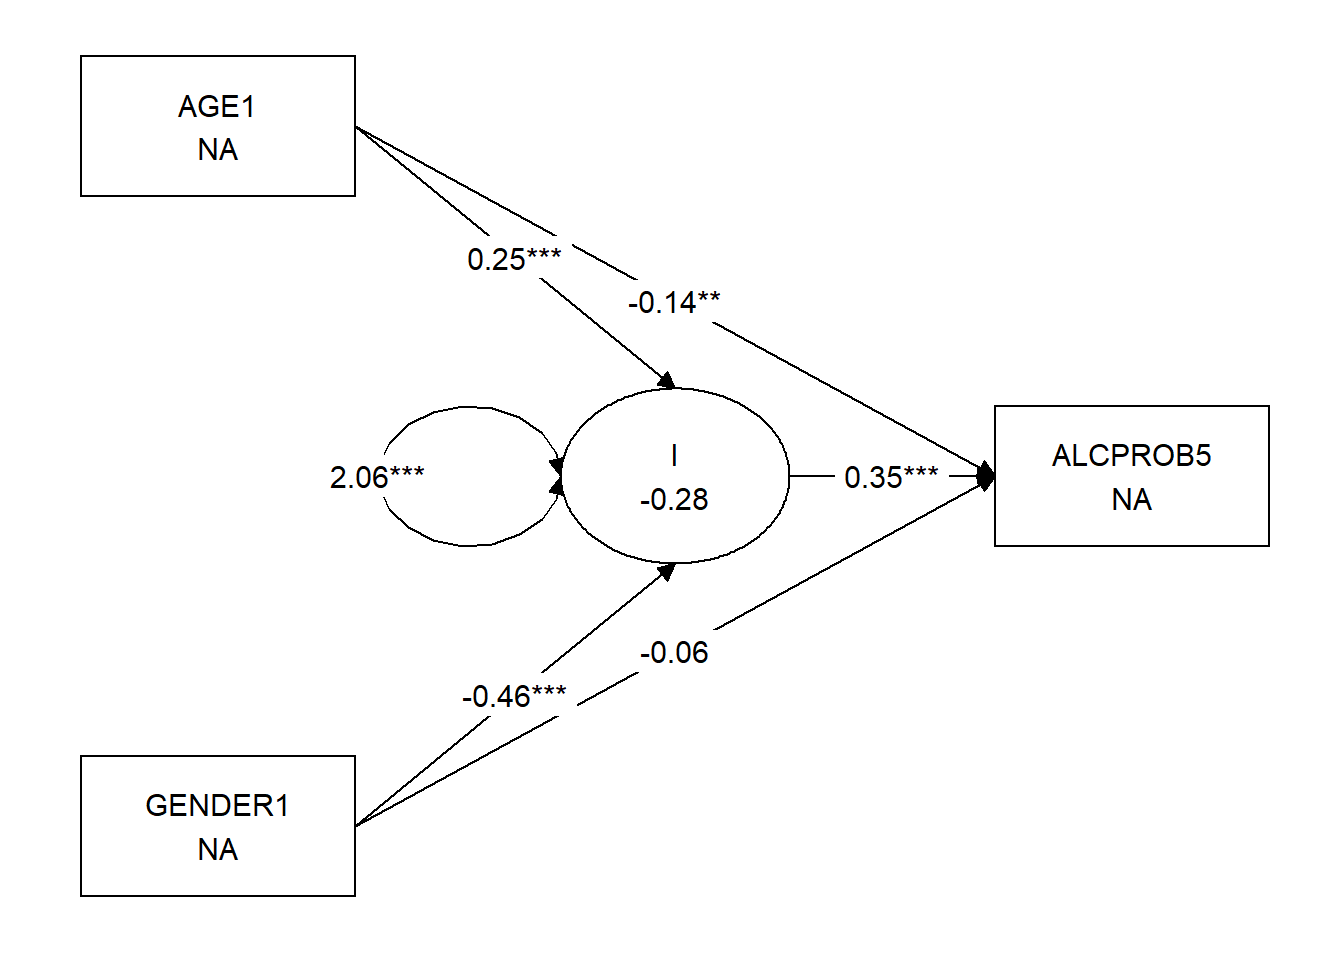
\includegraphics{S23_files/figure-latex/unnamed-chunk-18-1.pdf}

\hypertarget{exercise-3-level-and-shape-parameterization}{%
\section{Exercise 3: Level and Shape Parameterization}\label{exercise-3-level-and-shape-parameterization}}

The file GPA.dat holds the GPA data (GPA = grade point average) with GPA scores of 200 students in 6 consecutive
semesters. There are also time-invariant covariates: high school GPA and gender; and the outcome variable:
admitted to university of choice (missing if not applied for university). Use the GPA data to set up a level and shape
model.

First, load the data and name the variables:

\begin{Shaded}
\begin{Highlighting}[]
\NormalTok{data }\OtherTok{\textless{}{-}} \FunctionTok{read.table}\NormalTok{(}\StringTok{"GPA.dat"}\NormalTok{)}
\FunctionTok{names}\NormalTok{(data) }\OtherTok{\textless{}{-}} \FunctionTok{c}\NormalTok{(}\StringTok{"STUDENT"}\NormalTok{, }\StringTok{"SEX"}\NormalTok{, }\StringTok{"HIGHGPA"}\NormalTok{,}
                 \StringTok{"GPA1"}\NormalTok{, }\StringTok{"GPA2"}\NormalTok{, }\StringTok{"GPA3"}\NormalTok{, }\StringTok{"GPA4"}\NormalTok{, }\StringTok{"GPA5"}\NormalTok{, }\StringTok{"GPA6"}\NormalTok{)}
\end{Highlighting}
\end{Shaded}

\hypertarget{exercise-3a}{%
\subsection{Exercise 3a}\label{exercise-3a}}

Use a parameterization with \href{mailto:GPA1@0}{\nolinkurl{GPA1@0}} and \href{mailto:GPA6@1}{\nolinkurl{GPA6@1}}. The loadings for the other timepoints should be freely estimated. This can
be done with, for example, the syntax GPA2* as shown in the handout.\\
Interpret the factor loadings and estimate for S.

Click to show answers

This can be done as follows:

\begin{Shaded}
\begin{Highlighting}[]
\NormalTok{m3 }\OtherTok{\textless{}{-}} \FunctionTok{mplusObject}\NormalTok{(}
  \AttributeTok{MODEL =} \StringTok{"i s | gpa1@0 gpa2* gpa3* gpa4* gpa5* gpa6@1;"}\NormalTok{,}
  \AttributeTok{rdata =}\NormalTok{ data,}
  \AttributeTok{usevariables =} \FunctionTok{c}\NormalTok{(}\StringTok{"GPA1"}\NormalTok{, }\StringTok{"GPA2"}\NormalTok{, }\StringTok{"GPA3"}\NormalTok{, }\StringTok{"GPA4"}\NormalTok{, }\StringTok{"GPA5"}\NormalTok{, }\StringTok{"GPA6"}\NormalTok{),}
  \AttributeTok{modelout =} \StringTok{"m3.inp"}
\NormalTok{)}

\NormalTok{res }\OtherTok{\textless{}{-}} \FunctionTok{mplusModeler}\NormalTok{(m3, }\AttributeTok{run =}\NormalTok{ 1L)}

\CommentTok{\# Get all columns of results}
\NormalTok{tab }\OtherTok{\textless{}{-}} \FunctionTok{table\_results}\NormalTok{(res, }\AttributeTok{columns =} \ConstantTok{NULL}\NormalTok{)}
\CommentTok{\# Retain factor loadings and intercepts using op \%in\% c("=\textasciitilde{}", "\textasciitilde{}1") }
\CommentTok{\# for all parameters involving S (lhs == "S")}
\NormalTok{tab }\OtherTok{\textless{}{-}}\NormalTok{ tab[tab}\SpecialCharTok{$}\NormalTok{lhs }\SpecialCharTok{==} \StringTok{"S"} \SpecialCharTok{\&}\NormalTok{ tab}\SpecialCharTok{$}\NormalTok{op }\SpecialCharTok{\%in\%} \FunctionTok{c}\NormalTok{(}\StringTok{"=\textasciitilde{}"}\NormalTok{, }\StringTok{"\textasciitilde{}1"}\NormalTok{), ]}
\NormalTok{tab[, }\FunctionTok{c}\NormalTok{(}\StringTok{"label"}\NormalTok{, }\StringTok{"est\_sig"}\NormalTok{, }\StringTok{"pval"}\NormalTok{, }\StringTok{"confint"}\NormalTok{)]}
\end{Highlighting}
\end{Shaded}

\begin{tabular}[t]{l|l|l|l}
\hline
label & est\_sig & pval & confint\\
\hline
S.|.GPA1 & 0.00 & NA & NA\\
\hline
S.|.GPA2 & 0.24*** & 0.00 & [ 0.16,  0.32]\\
\hline
S.|.GPA3 & 0.45*** & 0.00 & [ 0.38,  0.52]\\
\hline
S.|.GPA4 & 0.65*** & 0.00 & [ 0.60,  0.70]\\
\hline
S.|.GPA5 & 0.81*** & 0.00 & [ 0.77,  0.86]\\
\hline
S.|.GPA6 & 1.00 & NA & NA\\
\hline
Means.S & 0.55*** & 0.00 & [ 0.49,  0.61]\\
\hline
\end{tabular}

\hypertarget{exercise-3b}{%
\subsection{Exercise 3b}\label{exercise-3b}}

Now use a parameterization with \href{mailto:GPA1@0}{\nolinkurl{GPA1@0}} and \href{mailto:GPA2@1}{\nolinkurl{GPA2@1}}. The other GPA's should be freely estimated.
Interpret the factor loadings and estimate for S.

Click to show answers

This can be done as follows:

\begin{Shaded}
\begin{Highlighting}[]
\NormalTok{m3b }\OtherTok{\textless{}{-}}\NormalTok{ m3 }
\NormalTok{m3b}\SpecialCharTok{$}\NormalTok{MODEL }\OtherTok{\textless{}{-}} \StringTok{"i s | gpa1@0 gpa2@1 gpa3* gpa4* gpa5* gpa6*;"}

\NormalTok{res\_3b }\OtherTok{\textless{}{-}} \FunctionTok{mplusModeler}\NormalTok{(m3b, }\AttributeTok{run =}\NormalTok{ 1L)}

\CommentTok{\# Get all columns of results}
\NormalTok{tab }\OtherTok{\textless{}{-}} \FunctionTok{table\_results}\NormalTok{(res\_3b, }\AttributeTok{columns =} \ConstantTok{NULL}\NormalTok{)}
\CommentTok{\# Retain factor loadings and intercepts using op \%in\% c("=\textasciitilde{}", "\textasciitilde{}1") }
\CommentTok{\# for all parameters involving S (lhs == "S")}
\NormalTok{tab }\OtherTok{\textless{}{-}}\NormalTok{ tab[tab}\SpecialCharTok{$}\NormalTok{lhs }\SpecialCharTok{==} \StringTok{"S"} \SpecialCharTok{\&}\NormalTok{ tab}\SpecialCharTok{$}\NormalTok{op }\SpecialCharTok{\%in\%} \FunctionTok{c}\NormalTok{(}\StringTok{"=\textasciitilde{}"}\NormalTok{, }\StringTok{"\textasciitilde{}1"}\NormalTok{), ]}
\NormalTok{tab[, }\FunctionTok{c}\NormalTok{(}\StringTok{"label"}\NormalTok{, }\StringTok{"est\_sig"}\NormalTok{, }\StringTok{"pval"}\NormalTok{, }\StringTok{"confint"}\NormalTok{)]}
\end{Highlighting}
\end{Shaded}

\begin{tabular}[t]{l|l|l|l}
\hline
label & est\_sig & pval & confint\\
\hline
S.|.GPA1 & 0.00 & NA & NA\\
\hline
S.|.GPA2 & 1.00 & NA & NA\\
\hline
S.|.GPA3 & 1.88*** & 0.00 & [ 1.31,  2.46]\\
\hline
S.|.GPA4 & 2.73*** & 0.00 & [ 1.89,  3.58]\\
\hline
S.|.GPA5 & 3.41*** & 0.00 & [ 2.33,  4.49]\\
\hline
S.|.GPA6 & 4.18*** & 0.00 & [ 2.82,  5.55]\\
\hline
Means.S & 0.13*** & 0.00 & [ 0.08,  0.18]\\
\hline
\end{tabular}

Which parameterization do you like best?

\hypertarget{exercise-3c}{%
\subsection{Exercise 3c}\label{exercise-3c}}

Draw the development of GPA over time based on your own calculations (by hand).
Compare this to the estimated means plot that you can get with the plot command:
PLOT: SERIES = GPA1-GPA6 (s);
TYPE = PLOT3;\\
However, don't forget that you need to `rescale' that plot, since S is linear while the location of the
estimated points is based on the factor loadings.

Click to show answers

This can be done as follows. Note that you will have to load the plot in Mplus:

\begin{Shaded}
\begin{Highlighting}[]
\NormalTok{m3b}\SpecialCharTok{$}\NormalTok{PLOT }\OtherTok{\textless{}{-}} \StringTok{"SERIES = GPA1{-}GPA6 (s);}
\StringTok{             TYPE = PLOT3;"}

\NormalTok{res\_3b }\OtherTok{\textless{}{-}} \FunctionTok{mplusModeler}\NormalTok{(m3b, }\AttributeTok{run =}\NormalTok{ 1L)}
\end{Highlighting}
\end{Shaded}

\hypertarget{exercise-3d}{%
\subsection{Exercise 3d}\label{exercise-3d}}

Use sex as a predictor of the intercept and slope and interpret the result (with 0 = boys, 1 = girls).

Click to show answers

This can be done as follows:

\begin{Shaded}
\begin{Highlighting}[]
\NormalTok{m3\_sex }\OtherTok{\textless{}{-}}\NormalTok{ m3}
\CommentTok{\# Make 0 = boys and 1 = girls}
\NormalTok{m3\_sex}\SpecialCharTok{$}\NormalTok{rdata}\SpecialCharTok{$}\NormalTok{SEX }\OtherTok{\textless{}{-}}\NormalTok{ m3\_sex}\SpecialCharTok{$}\NormalTok{rdata}\SpecialCharTok{$}\NormalTok{SEX }\SpecialCharTok{{-}} \DecValTok{1}
\NormalTok{m3\_sex}\SpecialCharTok{$}\NormalTok{usevariables }\OtherTok{\textless{}{-}} \FunctionTok{c}\NormalTok{(m3\_sex}\SpecialCharTok{$}\NormalTok{usevariables, }\StringTok{"SEX"}\NormalTok{)}
\NormalTok{m3\_sex}\SpecialCharTok{$}\NormalTok{MODEL }\OtherTok{\textless{}{-}} \FunctionTok{paste0}\NormalTok{(m3\_sex}\SpecialCharTok{$}\NormalTok{MODEL, }\StringTok{"i s on sex;"}\NormalTok{)}
\NormalTok{res\_3sex }\OtherTok{\textless{}{-}} \FunctionTok{mplusModeler}\NormalTok{(m3\_sex, }\AttributeTok{run =}\NormalTok{ 1L)}
\CommentTok{\# Get all columns of results}
\NormalTok{tab }\OtherTok{\textless{}{-}} \FunctionTok{table\_results}\NormalTok{(res\_3sex, }\AttributeTok{columns =} \ConstantTok{NULL}\NormalTok{)}
\CommentTok{\# Retain only regressions on I and S}
\NormalTok{tab }\OtherTok{\textless{}{-}}\NormalTok{ tab[tab}\SpecialCharTok{$}\NormalTok{lhs }\SpecialCharTok{\%in\%} \FunctionTok{c}\NormalTok{(}\StringTok{"I"}\NormalTok{, }\StringTok{"S"}\NormalTok{) }\SpecialCharTok{\&}\NormalTok{ tab}\SpecialCharTok{$}\NormalTok{op }\SpecialCharTok{==} \StringTok{"\textasciitilde{}"}\NormalTok{, ]}
\NormalTok{tab[, }\FunctionTok{c}\NormalTok{(}\StringTok{"label"}\NormalTok{, }\StringTok{"est\_sig"}\NormalTok{, }\StringTok{"pval"}\NormalTok{, }\StringTok{"confint"}\NormalTok{)]}
\end{Highlighting}
\end{Shaded}

\begin{tabular}[t]{l|l|l|l}
\hline
label & est\_sig & pval & confint\\
\hline
I.ON.SEX & 0.08* & 0.03 & [ 0.01,  0.15]\\
\hline
S.ON.SEX & 0.14* & 0.01 & [ 0.03,  0.24]\\
\hline
\end{tabular}

\hypertarget{exercise-4-latent-growth-model-on-gpa-data}{%
\section{Exercise 4: latent growth model on GPA data}\label{exercise-4-latent-growth-model-on-gpa-data}}

\hypertarget{exercise-4a}{%
\subsection{Exercise 4a}\label{exercise-4a}}

Continuing with the data used for the previous exercise, set up a latent growth model for GPA for the 6 consecutive occasions and run this model. Obtain the following parameters:

\begin{itemize}
\tightlist
\item
  AIC/BIC, Chi Square, RMSEA, CFI/TLI
\item
  Mean Intercept and Slope
\item
  Variance of the Intercept and Slope
\end{itemize}

Click to show answers

This can be done as follows, using m3 as starting point:

\begin{Shaded}
\begin{Highlighting}[]
\NormalTok{m4 }\OtherTok{\textless{}{-}}\NormalTok{ m3}
\NormalTok{m4}\SpecialCharTok{$}\NormalTok{MODEL }\OtherTok{\textless{}{-}} \StringTok{"i s | gpa1@0 gpa2@1 gpa3@2 gpa4@3 gpa5@4 gpa6@5;"}
\NormalTok{m4}\SpecialCharTok{$}\NormalTok{modelout }\OtherTok{\textless{}{-}} \StringTok{"m4.inp"}
\NormalTok{res\_4 }\OtherTok{\textless{}{-}} \FunctionTok{mplusModeler}\NormalTok{(m4, }\AttributeTok{run =}\NormalTok{ 1L)}
\CommentTok{\# Get the requested fit indices:}
\FunctionTok{get\_summaries}\NormalTok{(res\_4)[}\FunctionTok{c}\NormalTok{(}\StringTok{"AIC"}\NormalTok{, }\StringTok{"BIC"}\NormalTok{, }\StringTok{"ChiSqM\_Value"}\NormalTok{,}
                       \StringTok{"RMSEA\_Estimate"}\NormalTok{, }\StringTok{"CFI"}\NormalTok{, }\StringTok{"TLI"}\NormalTok{)]}
\CommentTok{\# Get all columns of results}
\NormalTok{tab }\OtherTok{\textless{}{-}} \FunctionTok{table\_results}\NormalTok{(res\_4, }\AttributeTok{columns =} \ConstantTok{NULL}\NormalTok{)}
\CommentTok{\# Retain only regressions on I and S}
\NormalTok{tab }\OtherTok{\textless{}{-}}\NormalTok{ tab[tab}\SpecialCharTok{$}\NormalTok{lhs }\SpecialCharTok{\%in\%} \FunctionTok{c}\NormalTok{(}\StringTok{"I"}\NormalTok{, }\StringTok{"S"}\NormalTok{) }\SpecialCharTok{\&}\NormalTok{ tab}\SpecialCharTok{$}\NormalTok{op }\SpecialCharTok{\%in\%} \FunctionTok{c}\NormalTok{(}\StringTok{"\textasciitilde{}\textasciitilde{}"}\NormalTok{, }\StringTok{"\textasciitilde{}1"}\NormalTok{), ]}
\NormalTok{tab[, }\FunctionTok{c}\NormalTok{(}\StringTok{"label"}\NormalTok{, }\StringTok{"est\_sig"}\NormalTok{, }\StringTok{"pval"}\NormalTok{, }\StringTok{"confint"}\NormalTok{)]}
\end{Highlighting}
\end{Shaded}

AIC BIC ChiSqM\_Value RMSEA\_Estimate CFI TLI
1 121 157 44 0.093 0.96 0.97

\begin{tabular}[t]{l|l|l|l}
\hline
label & est\_sig & pval & confint\\
\hline
S.WITH.I & 0.00 & 0.12 & [-0.00,  0.01]\\
\hline
Means.I & 2.60*** & 0.00 & [ 2.56,  2.63]\\
\hline
Means.S & 0.11*** & 0.00 & [ 0.10,  0.12]\\
\hline
Variances.I & 0.04*** & 0.00 & [ 0.02,  0.05]\\
\hline
Variances.S & 0.00*** & 0.00 & [ 0.00,  0.00]\\
\hline
\end{tabular}

\hypertarget{exercise-4b}{%
\subsection{Exercise 4b}\label{exercise-4b}}

Then, set up a latent growth model for 3 years where each year is a latent variable measured by the GPA of two
consecutive semesters.

The factor loadings for GPA2, GPA4 and GPA6 ought to be constrained to be equal with a label (a) behind
the loading in the syntax. As such, the scores relate in the same way to the year score over time. The GPA
intercepts are constrained at 0.

If you get the error message below, can you find out what the problem is?

\begin{verbatim}
WARNING:  THE LATENT VARIABLE COVARIANCE MATRIX (PSI) IS NOT POSITIVE     DEFINITE. THIS 
COULD INDICATE A NEGATIVE VARIANCE/RESIDUAL VARIANCE FOR A LATENT VARIABLE, A CORRELATION 
GREATER OR EQUAL TO ONE BETWEEN TWO LATENT VARIABLES, OR A LINEAR DEPENDENCY AMONG MORE 
THAN TWO LATENT VARIABLES. CHECK THE TECH4 OUTPUT FOR MORE INFORMATION. 
\end{verbatim}

A rough way to deal with this problem may be to fix the problematic parameter to a particular value (ie. .001), try this and re-run the model.

Now examine the same parameters as for exercise 3a, and compare the two. Are there
major differences?

\begin{itemize}
\tightlist
\item
  AIC/BIC, Chi Square, RMSEA, CFI/TLI
\item
  Mean Intercept and Slope
\item
  Variance of the Intercept and Slope
\end{itemize}

Click to show answers

This can be done as follows, using m3 as starting point:

\begin{Shaded}
\begin{Highlighting}[]
\NormalTok{m4b }\OtherTok{\textless{}{-}}\NormalTok{ m4}
\NormalTok{m4b}\SpecialCharTok{$}\NormalTok{MODEL }\OtherTok{\textless{}{-}} \StringTok{"year1 by gpa1@1 gpa2 (a);}
\StringTok{             year2 by gpa3@1 gpa4 (a); }
\StringTok{             year3 by gpa5@1 gpa6 (a);}
\StringTok{             [gpa1@0 gpa2@0 gpa3@0 gpa4@0 gpa5@0 gpa6@0];}
\StringTok{             i s | year1@0 year2@1 year3@2;}
\StringTok{             [i s];}
\StringTok{             year3@.001;"}
\NormalTok{res\_4b }\OtherTok{\textless{}{-}} \FunctionTok{mplusModeler}\NormalTok{(m4b, }\AttributeTok{run =}\NormalTok{ 1L)}
\CommentTok{\# Get the requested fit indices:}
\FunctionTok{get\_summaries}\NormalTok{(res\_4b)[}\FunctionTok{c}\NormalTok{(}\StringTok{"AIC"}\NormalTok{, }\StringTok{"BIC"}\NormalTok{, }\StringTok{"ChiSqM\_Value"}\NormalTok{,}
                        \StringTok{"RMSEA\_Estimate"}\NormalTok{, }\StringTok{"CFI"}\NormalTok{, }\StringTok{"TLI"}\NormalTok{)]}
\CommentTok{\# Get all columns of results}
\NormalTok{tab }\OtherTok{\textless{}{-}} \FunctionTok{table\_results}\NormalTok{(res\_4b, }\AttributeTok{columns =} \ConstantTok{NULL}\NormalTok{)}
\CommentTok{\# Retain only regressions on I and S}
\NormalTok{tab }\OtherTok{\textless{}{-}}\NormalTok{ tab[tab}\SpecialCharTok{$}\NormalTok{lhs }\SpecialCharTok{\%in\%} \FunctionTok{c}\NormalTok{(}\StringTok{"I"}\NormalTok{, }\StringTok{"S"}\NormalTok{) }\SpecialCharTok{\&}\NormalTok{ tab}\SpecialCharTok{$}\NormalTok{op }\SpecialCharTok{\%in\%} \FunctionTok{c}\NormalTok{(}\StringTok{"\textasciitilde{}\textasciitilde{}"}\NormalTok{, }\StringTok{"\textasciitilde{}1"}\NormalTok{), ]}
\NormalTok{tab[, }\FunctionTok{c}\NormalTok{(}\StringTok{"label"}\NormalTok{, }\StringTok{"est\_sig"}\NormalTok{, }\StringTok{"pval"}\NormalTok{, }\StringTok{"confint"}\NormalTok{)]}
\end{Highlighting}
\end{Shaded}

AIC BIC ChiSqM\_Value RMSEA\_Estimate CFI TLI
1 130 177 48 0.12 0.96 0.95

\begin{tabular}[t]{l|l|l|l}
\hline
label & est\_sig & pval & confint\\
\hline
S.WITH.I & 0.01*** & 0.00 & [ 0.01,  0.02]\\
\hline
Means.I & 2.60*** & 0.00 & [ 2.56,  2.64]\\
\hline
Means.S & 0.21*** & 0.00 & [ 0.19,  0.23]\\
\hline
Variances.I & 0.03*** & 0.00 & [ 0.02,  0.04]\\
\hline
Variances.S & 0.01** & 0.00 & [ 0.00,  0.01]\\
\hline
\end{tabular}

\hypertarget{day-3-latent-growth-mixture-modeling}{%
\chapter{Day 3: Latent Growth (Mixture) Modeling}\label{day-3-latent-growth-mixture-modeling}}

This computer lab session demonstrates to run latent growth mixture models in batch, using the R-package \texttt{MplusAutomation}.
Note that, if you do not want to automate part of your workflow (like making plots and tables), you can also use Mplus exclusively.
All of the input files for the exercises described in this GitBook are provided with the course materials.

To get started with today's computer lab, first open the project file called ``S23.Rproj.'' It should load in the program ``RStudio.'' The bottom right panel has several tabs, including one called ``Files.'' Click on ``Files'' in this bottom right tab, and click the file ``mixture\_exercises.R.''

This computer lab session demonstrates to run latent growth models in batch, using the R-package \texttt{MplusAutomation}.
Note that, if you do not want to automate part of your workflow (like making plots and tables), you can also use Mplus exclusively.
All of the input files for the exercises described in this GitBook are provided with the course materials.

To get started with today's computer lab, first open the project file called ``S23.Rproj.'' It should load in the program ``RStudio.'' The bottom right panel has several tabs, including one called ``Files.'' Click on ``Files'' in this bottom right tab, and click the file ``growth\_exercises.R.''

\hypertarget{exercise-1-latent-growth-mixture-modeling}{%
\section{Exercise 1: Latent Growth (Mixture) Modeling}\label{exercise-1-latent-growth-mixture-modeling}}

\hypertarget{a.-latent-class-growth-models.}{%
\subsection{1a. Latent Class Growth Models.}\label{a.-latent-class-growth-models.}}

Set up the growth curve model as depicted in Figure 1 in Mplus, using the \textbar{} notation. Use the file DDS8\_1.dat for this.

\begin{figure}
\centering
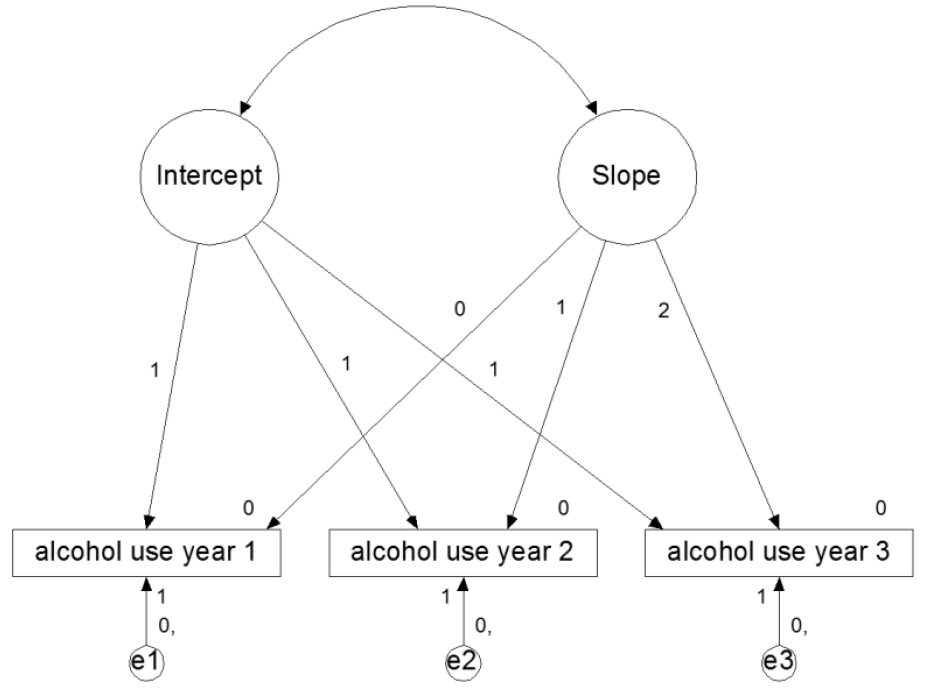
\includegraphics[width=4.16667in,height=\textheight]{./Materials/Figure1_lgm_alcohol.png}
\caption{Latent Growth model for alcohol}
\end{figure}

First, load the file \texttt{DDS8\_1.dat} into the R environment. For convenience's sake, rename the columns of the data object to something a human would understand:

\begin{Shaded}
\begin{Highlighting}[]
\NormalTok{data }\OtherTok{\textless{}{-}} \FunctionTok{read.table}\NormalTok{(}\StringTok{"DDS8\_1.dat"}\NormalTok{, }\AttributeTok{na.strings =} \SpecialCharTok{{-}}\DecValTok{99}\NormalTok{)}
\FunctionTok{names}\NormalTok{(data) }\OtherTok{\textless{}{-}} \FunctionTok{c}\NormalTok{(}\StringTok{"ALC1YR1"}\NormalTok{, }\StringTok{"ALC1YR2"}\NormalTok{, }\StringTok{"ALC1YR3"}\NormalTok{,}
                 \StringTok{"ALCPROB5"}\NormalTok{, }\StringTok{"AGE1"}\NormalTok{, }\StringTok{"GENDER1"}\NormalTok{)}
\end{Highlighting}
\end{Shaded}

Use the function \texttt{createMixtures} to define the latent class growth model as displayed in Figure 1. To see how the function \texttt{createMixtures()} works, type its name, select it, and press F1.

You can specify the model using the ``\textbar{}'' notation. Constrain the variance of the intercept and slope factors to be equal to zero, using the Mplus syntax \texttt{i@0;\ s@0;}.

In createMixtures, you can specify the overall model using the argument \texttt{model\_overall\ =\ "i\ s\ \textbar{}\ ALC1YR1@0\ ALC1YR2@1\ ALC1YR3@2;\ \ i@0;\ \ s@0;"}. The double spaces are converted to newline characters, which results in a nicely formatted Mplus file.

Request 1 to 6 classes, by specifying the argument \texttt{classes\ =\ 1:6} for createMixtures. Request tech8, tech11 and tech14 output by specifying the argument: \texttt{OUTPUT\ =\ "tech8\ tech11\ tech14;"}.

To run the analysis, add the argument \texttt{run\ =\ 1L} to the \texttt{createMixtures()} call.
Make sure to store the resulting output in an object, the same way you stored the data in an object called \texttt{data} when using the function \texttt{read.table()}.

Click to show answers

The resulting syntax should look like this:

\begin{Shaded}
\begin{Highlighting}[]
\NormalTok{results\_1a }\OtherTok{\textless{}{-}} \FunctionTok{createMixtures}\NormalTok{(}
  \AttributeTok{classes =} \DecValTok{1}\SpecialCharTok{:}\DecValTok{6}\NormalTok{,}
  \AttributeTok{filename\_stem =} \StringTok{"1a"}\NormalTok{,}
  \AttributeTok{model\_overall =} \StringTok{"i s | ALC1YR1@0 ALC1YR2@1 ALC1YR3@2;}
\StringTok{                   i@0;  s@0;"}\NormalTok{,}
  \AttributeTok{rdata =}\NormalTok{ data, }
  \AttributeTok{usevariables =} \FunctionTok{c}\NormalTok{(}\StringTok{"ALC1YR1"}\NormalTok{, }\StringTok{"ALC1YR2"}\NormalTok{, }\StringTok{"ALC1YR3"}\NormalTok{),}
  \AttributeTok{OUTPUT =} \StringTok{"tech8 tech11 tech14;"}\NormalTok{,}
  \AttributeTok{run =}\NormalTok{ 1L)}
\end{Highlighting}
\end{Shaded}

The function \texttt{createModels()} can run all of the analyses in batch, thus taking a lot of work out of your hands.
The function essentially performs three steps:

\begin{enumerate}
\def\labelenumi{\arabic{enumi}.}
\tightlist
\item
  Create Mplus syntax for each of the latent class models based on \texttt{model\_overall} and \texttt{model\_class\_specific}
\item
  Use the function \texttt{mplusObject()} to turn this syntax into a model that can be evaluated
\item
  Use the function \texttt{mplusModeler()} to create the Mplus \texttt{.inp} files, run them, and return the results
\end{enumerate}

If you use MplusAutomation for other types of models, you won't need \texttt{createMixtures()}. Instead, you can use \texttt{mplusObject()} and \texttt{mplusModeler()}.

To see what the function \texttt{createMixtures()} is doing, you should inspect each of the automatically generated input files (\texttt{.inp}). You can even run one by hand.

Finally, print a summary table to the R console by calling \texttt{mixtureSummaryTable()} on the results object.

Click to show answers

The resulting syntax should look like this:

\begin{Shaded}
\begin{Highlighting}[]
\FunctionTok{mixtureSummaryTable}\NormalTok{(results\_1a)}
\end{Highlighting}
\end{Shaded}

\begin{tabular}[t]{l|r|r|r|r|r|r|r|r|r|r|r|r}
\hline
Title & Classes & AIC & BIC & aBIC & Entropy & T11\_VLMR\_PValue & T11\_LMR\_PValue & BLRT\_PValue & min\_N & max\_N & min\_prob & max\_prob\\
\hline
6 classes & 1 & 4938 & 5020 & 4957 & 0.76 & 0.00 & 0.00 & 0 & 466 & 466 & 1.00 & 1.00\\
\hline
5 classes & 2 & 4962 & 5032 & 4978 & 0.75 & 0.11 & 0.12 & 0 & 144 & 322 & 0.86 & 0.95\\
\hline
4 classes & 3 & 4971 & 5029 & 4984 & 0.80 & 0.01 & 0.01 & 0 & 65 & 262 & 0.86 & 0.96\\
\hline
3 classes & 4 & 4995 & 5040 & 5005 & 0.82 & 0.00 & 0.00 & 0 & 39 & 237 & 0.65 & 0.94\\
\hline
2 classes & 5 & 5191 & 5224 & 5199 & 0.73 & 0.00 & 0.00 & 0 & 34 & 204 & 0.73 & 0.92\\
\hline
1 classes & 6 & 5339 & 5360 & 5344 & NA & NA & NA & NA & 32 & 147 & 0.69 & 0.91\\
\hline
\end{tabular}

\hypertarget{visualization-1}{%
\subsubsection{Visualization}\label{visualization-1}}

To verify that the estimated model corresponds to the Figure above, you can use the SEM graphing package \texttt{tidySEM}.
This flexible package produces fully customizable plots based on the R graphing package \texttt{ggplot2} for Mplus (and \texttt{lavaan}) models.
If you want to make publication quality graphs, \href{https://cjvanlissa.github.io/tidySEM/articles/Plotting_graphs.html}{here is an online tutorial for graph customization}.
The script below demonstrates how to plot a model using \texttt{tidySEM}.

\begin{Shaded}
\begin{Highlighting}[]
\FunctionTok{install.packages}\NormalTok{(}\StringTok{"tidySEM"}\NormalTok{)}
\FunctionTok{library}\NormalTok{(tidySEM)}
\NormalTok{lo }\OtherTok{\textless{}{-}} \FunctionTok{get\_layout}\NormalTok{(}\StringTok{"I"}\NormalTok{,       }\StringTok{""}\NormalTok{,        }\StringTok{"S"}\NormalTok{,}
                 \StringTok{"ALC1YR1"}\NormalTok{, }\StringTok{"ALC1YR2"}\NormalTok{, }\StringTok{"ALC1YR3"}\NormalTok{, }\AttributeTok{rows =} \DecValTok{2}\NormalTok{)}
\FunctionTok{graph\_sem}\NormalTok{(results\_1a[[}\DecValTok{1}\NormalTok{]], }\AttributeTok{layout =}\NormalTok{ lo, }\AttributeTok{angle =} \DecValTok{179}\NormalTok{)}
\end{Highlighting}
\end{Shaded}

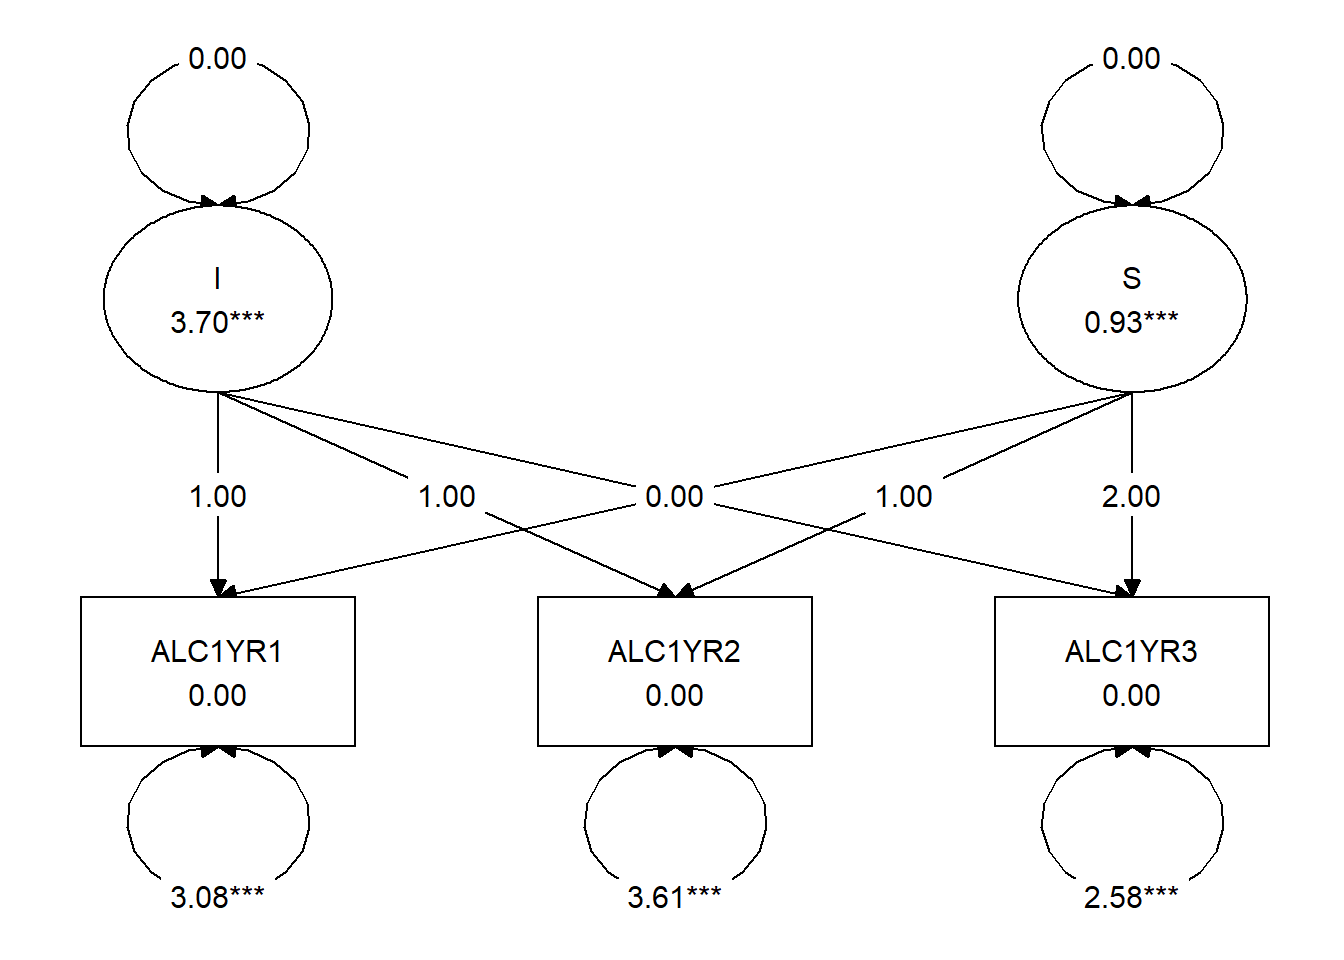
\includegraphics{S23_files/figure-latex/demotidysem-1.pdf}

\hypertarget{b.-increasing-random-starts}{%
\subsection{1b. Increasing random starts}\label{b.-increasing-random-starts}}

These models use random starting values. Several independent random starts are made, to ensure that the model converges on the proper solution. The default is 20 random sets of starting values, of which 4 are run to completion. Inspect the output, and look carefully if the model estimation has converged, especially for the larger number of classes. Look for warning and error messages, make sure you understand what they are telling you.

The STARTS option is used to specify the number of initial random starting values and final stage optimizations. Now, increase the number of starts to ensure proper convergence. For createMixtures, the argument is \texttt{ANALYSIS\ =\ "STARTS\ =\ ..\ ..;"}.

Click to show answers

The resulting syntax should look like this:

\begin{Shaded}
\begin{Highlighting}[]
\NormalTok{results\_1b }\OtherTok{\textless{}{-}} 
  \FunctionTok{createMixtures}\NormalTok{(}\AttributeTok{classes =} \DecValTok{1}\SpecialCharTok{:}\DecValTok{6}\NormalTok{,}
                 \AttributeTok{filename\_stem =} \StringTok{"1b"}\NormalTok{,}
                 \AttributeTok{model\_overall =} \StringTok{"i s | ALC1YR1@0 ALC1YR2@1 ALC1YR3@2;}
\StringTok{                                  i@0;  s@0;"}\NormalTok{,}
                 \AttributeTok{ANALYSIS =} \StringTok{"STARTS = 50 10;"}\NormalTok{,}
                 \AttributeTok{rdata =}\NormalTok{ data, }
                 \AttributeTok{usevariables =} \FunctionTok{c}\NormalTok{(}\StringTok{"ALC1YR1"}\NormalTok{, }\StringTok{"ALC1YR2"}\NormalTok{, }\StringTok{"ALC1YR3"}\NormalTok{),}
                 \AttributeTok{OUTPUT =} \StringTok{"tech8 tech11 tech14;"}\NormalTok{,}
                 \AttributeTok{run =}\NormalTok{ 1L)}
\end{Highlighting}
\end{Shaded}

Make a mixture summary table to compare the fit information of the models with 1-6 classes, with the increased number of starts, using \texttt{mixtureSummaryTable()}. Also open the output files, and inspect the estimates in each class. Which model do you prefer, and why?

Click to show answers

The resulting syntax should look like this:

\begin{Shaded}
\begin{Highlighting}[]
\FunctionTok{mixtureSummaryTable}\NormalTok{(results\_1b)}
\end{Highlighting}
\end{Shaded}

\begin{tabular}[t]{l|r|r|r|r|r|r|r|r|r|r|r|r}
\hline
Title & Classes & AIC & BIC & aBIC & Entropy & T11\_VLMR\_PValue & T11\_LMR\_PValue & BLRT\_PValue & min\_N & max\_N & min\_prob & max\_prob\\
\hline
6 classes & 1 & 4938 & 5020 & 4957 & 0.76 & 0.00 & 0.00 & 0 & 466 & 466 & 1.00 & 1.00\\
\hline
5 classes & 2 & 4962 & 5032 & 4978 & 0.75 & 0.11 & 0.12 & 0 & 144 & 322 & 0.86 & 0.95\\
\hline
4 classes & 3 & 4971 & 5029 & 4984 & 0.80 & 0.01 & 0.01 & 0 & 65 & 262 & 0.86 & 0.96\\
\hline
3 classes & 4 & 4995 & 5040 & 5005 & 0.82 & 0.00 & 0.00 & 0 & 39 & 237 & 0.65 & 0.94\\
\hline
2 classes & 5 & 5191 & 5224 & 5199 & 0.73 & 0.00 & 0.00 & 0 & 34 & 204 & 0.73 & 0.92\\
\hline
1 classes & 6 & 5339 & 5360 & 5344 & NA & NA & NA & NA & 32 & 147 & 0.69 & 0.91\\
\hline
\end{tabular}

Based on the table, I would select a 3-class model. The fit indices and (V)LMR tests essentially indicate that you can keep adding classes and improve the model, which makes it difficult to decide. However, if we look at min\_N, we see that from 4 classes onward, the smallest class has less than 10\% of cases assigned to it. The minimum posterior classification probability and entropy are best for the 3-class model, which means that this model can reasonably accurately assign individuals to classes.

\hypertarget{c.-latent-growth-mixture-models.}{%
\subsection{1c. Latent Growth Mixture Models.}\label{c.-latent-growth-mixture-models.}}

Set up the same models as analyzed in the previous exercise, but now allow the means and variances of the intercept and slope factors to be freely estimated in each class. You do this by mentioning the intercept and slope explicitly in the class-specific part of the syntax. This is a more complex model, and we might therefore expect that we will need fewer classes for a good description of the data. This analysis will also take more computing time, so add \texttt{PROCESSORS=4} to the analysis section. Make a table of the fit indices, look at AIC, BIC, and the Bootstrapped LRT value (Tech 14).

Click to show answers

The resulting syntax should look like this:

\begin{Shaded}
\begin{Highlighting}[]
\NormalTok{results\_1c }\OtherTok{\textless{}{-}}
  \FunctionTok{createMixtures}\NormalTok{(}\AttributeTok{classes =} \DecValTok{1}\SpecialCharTok{:}\DecValTok{4}\NormalTok{,}
                 \AttributeTok{filename\_stem =} \StringTok{"1c"}\NormalTok{, }
                 \AttributeTok{model\_overall =} \StringTok{"i s | ALC1YR1@0 ALC1YR2@1 ALC1YR3@2;}
\StringTok{                                  i@0;  s@0;"}\NormalTok{,}
                 \AttributeTok{model\_class\_specific =} \StringTok{"i;  s;"}\NormalTok{,}
                 \AttributeTok{rdata =}\NormalTok{ data,}
                 \AttributeTok{OUTPUT =} \StringTok{"tech8 tech11 tech14;"}\NormalTok{,}
                 \AttributeTok{usevariables =} \FunctionTok{c}\NormalTok{(}\StringTok{"ALC1YR1"}\NormalTok{, }\StringTok{"ALC1YR2"}\NormalTok{, }\StringTok{"ALC1YR3"}\NormalTok{),}
                 \AttributeTok{ANALYSIS =} \StringTok{"PROCESSORS = 4;"}\NormalTok{,}
                 \AttributeTok{run =}\NormalTok{ 1L)}
\end{Highlighting}
\end{Shaded}

\hypertarget{d.-visualizing-growth-models.}{%
\subsection{1d. Visualizing growth models.}\label{d.-visualizing-growth-models.}}

Plotting the model-predicted trajectories makes it easier to interpret the model. Moreover, visualizing the raw data provides yet another way to evaluate the fit of your mixture model to the data. With this in mind, plot the four models you created in exercise \emph{1c}, and interpret what you see. First, plot only the predicted trajectories. Then, plot raw data as well. Explain the benefit of plotting the raw data in your own words.

\textit{Tip:} Because the scales in the alcohol data are ordinal, many of the observed trajectories overlap. To prevent `overplotting,' you can jitter the observed trajectories by a fraction of their standard deviation. Even as little as jitter\_lines = .1, jittering the positions on the y-axis by 1/10th of a standard deviation, can make a difference.

Click to show answers

Plotting the raw data helps us understand how representative the average trajectory for each class captures the individual trajectories of individuals in that class. It helps us see how separable the classes are visually, instead of just relying on statistics like entropy.

The resulting plot should look like this:

\begin{Shaded}
\begin{Highlighting}[]
\FunctionTok{plotGrowthMixtures}\NormalTok{(results\_1c, }\AttributeTok{rawdata =} \ConstantTok{TRUE}\NormalTok{, }\AttributeTok{jitter\_lines =}\NormalTok{ .}\DecValTok{1}\NormalTok{)}
\end{Highlighting}
\end{Shaded}

\begin{center}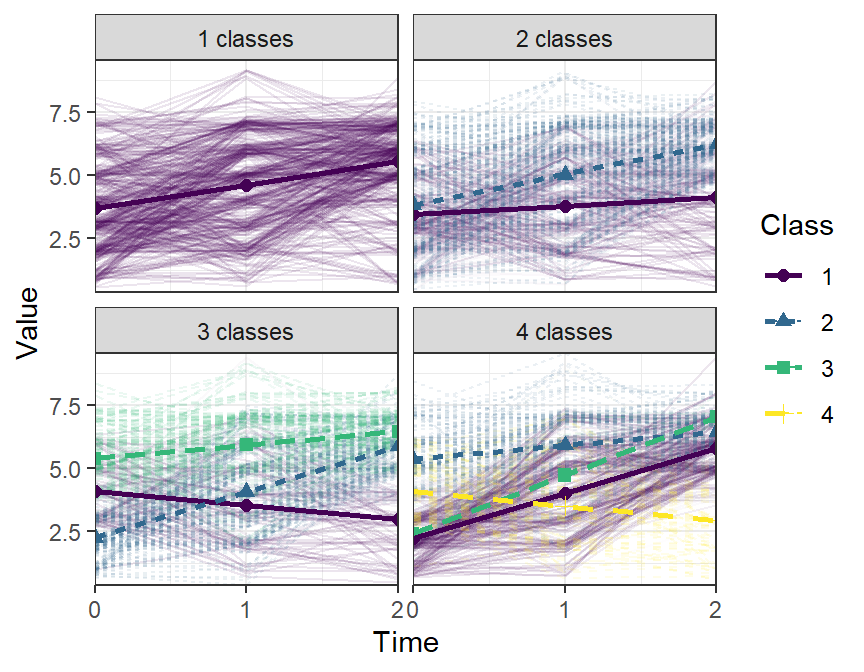
\includegraphics{S23_files/figure-latex/plot_gmm-1} \end{center}

\hypertarget{e.-the-3-step-model.}{%
\subsection{1e. The 3-step model.}\label{e.-the-3-step-model.}}

Covariates are often added to mixture models, to predict 1) class membership 2) to explain variation in the growth parameters within the classes or 3) as a distal outcome.

Whenever covariates are however added to the model, they change the Latent Class solution. Sometimes, this is fine, as the covariates can help to improve the classification. In other cases, you would use a 3-step approach, which Mplus has automated:

\begin{enumerate}
\def\labelenumi{\arabic{enumi}.}
\tightlist
\item
  Fit an unconditional Latent Class Model (without covariates)
\item
  A ``most likely class variable'' is created using the posterior distribution of step 1.
\item
  This most likely class variable is then regressed on (a) covariate.
\end{enumerate}

There are a few options for how to do 3-step analysis. They all rely on adding to the \texttt{Variable:} command.
For more info, see \url{https://www.statmodel.com/download/webnotes/webnote15.pdf}.

\hypertarget{commands-for-conducting-a-3-step-model}{%
\subsubsection{Commands for conducting a 3-step model}\label{commands-for-conducting-a-3-step-model}}

You can add the following options to the \texttt{Variable:} command:

\begin{enumerate}
\def\labelenumi{\arabic{enumi}.}
\tightlist
\item
  \texttt{Auxiliary\ =\ x(R);}~\\
  This is actually a 1-step method for predicting latent class memberships using Pseudo-Class draws.
\item
  \texttt{Auxiliary\ =\ x(R3step);}~\\
  A 3 step procedure, where covariates predict the latent class
\item
  \texttt{Auxiliary\ =\ y(e)}~\\
  A 1-step method, where the latent class predicts a continuous distal outcome.
\item
  \texttt{Auxiliary\ =\ y(de3step);}~\\
  A 3 step procedure, where latent class predicts continuous covariates (distal outcome) with unequal means and equal variances
\item
  \texttt{Auxiliary\ =\ y(du3step);}~\\
  A 3 step procedure, where latent class predicts continuous covariates (distal outcome) with unequal means and variances
\item
  \texttt{Auxiliary\ =\ Y(dcon);}~\\
  Procedure for continuous distal outcomes as suggested by Lanza et al (2013)
\item
  \texttt{Auxiliary\ =\ Y(dcon);}~\\
  Procedure for categorical distal outcomes as suggested by Lanza et al (2013)
\item
  \texttt{Auxiliary\ =\ y(BCH);}~\\
  Improved and currently best 3-step procedure with continuous covariates as distal outcomes
\end{enumerate}

Pick your final model from 1c, and add both age and gender as auxiliary variables in the model. Try to think what 3-step model you want, and if you are not sure, run different models, so you can evaluate how the different procedures make a difference. You can do this by editing the Mplus file, or by adding the \texttt{VARIABLE\ =\ "Auxiliary\ =\ ...;",} to your call to \texttt{createMixtures()}. What is the effect of both age and gender?

\emph{Note: The results can be extracted using the} \texttt{get\_lcCondMeans()} \emph{function.}

Click to show answers

I'm providing an example using the BCH 3-step procedure below. It can be seen, from the overall test and the pairwise comparisons, that the third group is significantly older, and has a significantly lower proportion of girls than the other two classes.

The resulting syntax and output should look like this:

\begin{Shaded}
\begin{Highlighting}[]
\NormalTok{results\_1e }\OtherTok{\textless{}{-}}
  \FunctionTok{createMixtures}\NormalTok{(}\AttributeTok{classes =} \DecValTok{3}\NormalTok{,}
                 \AttributeTok{filename\_stem =} \StringTok{"1e"}\NormalTok{, }
                 \AttributeTok{model\_overall =} \StringTok{"i s | ALC1YR1@0 ALC1YR2@1 ALC1YR3@2;}
\StringTok{                                  i@0;  s@0;"}\NormalTok{,}
                 \AttributeTok{model\_class\_specific =} \StringTok{"i;  s;"}\NormalTok{,}
                 \AttributeTok{rdata =}\NormalTok{ data,}
                 \AttributeTok{OUTPUT =} \StringTok{"tech8 tech11 tech14;"}\NormalTok{,}
                 \AttributeTok{usevariables =} \FunctionTok{c}\NormalTok{(}\StringTok{"ALC1YR1"}\NormalTok{, }\StringTok{"ALC1YR2"}\NormalTok{, }\StringTok{"ALC1YR3"}\NormalTok{,}
                                  \StringTok{"AGE1"}\NormalTok{, }\StringTok{"GENDER1"}\NormalTok{),}
                 \AttributeTok{VARIABLE =} \StringTok{"Auxiliary = AGE1(BCH)  GENDER1(BCH);"}\NormalTok{,}
                 \AttributeTok{ANALYSIS =} \StringTok{"PROCESSORS = 4;"}\NormalTok{,}
                 \AttributeTok{run =}\NormalTok{ 1L)}

\CommentTok{\# The results of the conditional means test are inside the output object}
\CommentTok{\# But you have to dig a little bit. The code to get them is:}
\FunctionTok{get\_lcCondMeans}\NormalTok{(results\_1e)}
\end{Highlighting}
\end{Shaded}

\begin{verbatim}
## $overall
##       var   m.1  se.1   m.2  se.2  m.3  se.3 chisq df     p
## 1    AGE1 14.81 0.227 15.31 0.114 15.9 0.107  25.7  2     0
## 2 GENDER1  0.48 0.063  0.46 0.037  0.3 0.042 9.421  2 0.009
## 
## $pairwise
##       var classA classB chisq df     p
## 1    AGE1      1      2  3.56 NA 0.059
## 2    AGE1      1      3 18.34 NA 0.000
## 3    AGE1      2      3 15.46 NA 0.000
## 4 GENDER1      1      2  0.11 NA 0.741
## 5 GENDER1      1      3  5.56 NA 0.018
## 6 GENDER1      2      3  7.79 NA 0.005
## 
## attr(,"class")
## [1] "mplus.auxE" "list"
\end{verbatim}

\hypertarget{exercise-2-latent-transition-analysis-lta}{%
\section{Exercise 2: Latent Transition Analysis (LTA)}\label{exercise-2-latent-transition-analysis-lta}}

\hypertarget{a.-latent-transition-analysis-with-probability-parameterization}{%
\subsection{2a. Latent transition analysis with probability parameterization}\label{a.-latent-transition-analysis-with-probability-parameterization}}

The file DatingSex.dat holds data on five indicators measured at two occasions (see MPlus example on LTA in user guide), as well as the variable gender. Read the file into memory, and name the variables:

\begin{Shaded}
\begin{Highlighting}[]
\NormalTok{data }\OtherTok{\textless{}{-}} \FunctionTok{read.table}\NormalTok{(}\StringTok{"DatingSex.dat"}\NormalTok{, }\AttributeTok{na.strings =} \SpecialCharTok{{-}}\DecValTok{99}\NormalTok{)}
\FunctionTok{names}\NormalTok{(data) }\OtherTok{\textless{}{-}} \FunctionTok{c}\NormalTok{(}\StringTok{"u11"}\NormalTok{, }\StringTok{"u12"}\NormalTok{, }\StringTok{"u13"}\NormalTok{, }\StringTok{"u14"}\NormalTok{, }\StringTok{"u15"}\NormalTok{, }
                 \StringTok{"u21"}\NormalTok{, }\StringTok{"u22"}\NormalTok{, }\StringTok{"u23"}\NormalTok{, }\StringTok{"u24"}\NormalTok{, }\StringTok{"u25"}\NormalTok{, }
                 \StringTok{"gender"}\NormalTok{)}
\end{Highlighting}
\end{Shaded}

The u-variables represent five yes/no items (second digit represents the item) measured at two time points (first digit represents time point). Set up a model with two latent class variables for the two time points. Exclude the variable gender for now. Assume there are 2 latent classes.

Set up and run a model that restricts the thresholds (and hence response probabilities) across the two time points by first repeating the thresholds for each Latent Class (2), in both Model C1: and Model C2. To be sure Mplus does what you want, include equality constraints on the five thresholds of c1\#1 and c2\#1, and similarly for c1\#2 and c2\#2. Use the lecture slides for help in specifying the model. Check the Mplus input files manually.

Using MplusAutomation, the model can be specified as follows:

\begin{Shaded}
\begin{Highlighting}[]
\NormalTok{results\_2a }\OtherTok{\textless{}{-}}
\FunctionTok{createMixtures}\NormalTok{(}
\CommentTok{\# Create only one model, with two classes}
\AttributeTok{classes =} \DecValTok{2}\NormalTok{,}
\CommentTok{\# Name the generated files "2a"}
\AttributeTok{filename\_stem =} \StringTok{"2a"}\NormalTok{,}
\CommentTok{\# Specify the autoregressive effect}
\AttributeTok{model\_overall =} \StringTok{"c2 ON c1;"}\NormalTok{,}
\CommentTok{\# Specify two class{-}specific models;}
\CommentTok{\# one for each categorical latent variable}
\AttributeTok{model\_class\_specific =} \FunctionTok{c}\NormalTok{(}
\StringTok{"[u11$1] (a\{C\});  [u12$1] (b\{C\});  [u13$1] (c\{C\});}
\StringTok{ [u14$1] (d\{C\});  [u15$1] (e\{C\});"}\NormalTok{,}
\StringTok{"[u21$1] (a\{C\});  [u22$1] (b\{C\});  [u23$1] (c\{C\});}
\StringTok{ [u24$1] (d\{C\});  [u25$1] (e\{C\});"}
\NormalTok{),}
\AttributeTok{rdata =}\NormalTok{ data,}
\AttributeTok{usevariables =} \FunctionTok{names}\NormalTok{(data)[}\SpecialCharTok{{-}}\DecValTok{11}\NormalTok{],}
\CommentTok{\# Speed up analysis by using 2 processors; increase random starts}
\CommentTok{\# Use probability parametrerization}
\AttributeTok{ANALYSIS =} \StringTok{"PROCESSORS IS 2;  LRTSTARTS (0 0 40 20);}
\StringTok{            PARAMETERIZATION = PROBABILITY;"}\NormalTok{,}
\CommentTok{\# Specify that the items are categorical (binary)}
\AttributeTok{VARIABLE =} \StringTok{"CATEGORICAL = u11{-}u15 u21{-}u25;"}\NormalTok{,}
\AttributeTok{run =}\NormalTok{ 1L}
\NormalTok{)}
\end{Highlighting}
\end{Shaded}

After running the analysis, inspect the proportions of yes/no answers for each of the indicators in the latent classes (look at probability scale in Mplus output).

Click to show answers

You can easily extract the parameters in probability scale from the output, using the \$ sign. They will be printed to the console as a table.

Here, we examine just the first few rows of the table:

\begin{Shaded}
\begin{Highlighting}[]
\NormalTok{results\_2a}\SpecialCharTok{$}\NormalTok{results}\SpecialCharTok{$}\NormalTok{parameters}\SpecialCharTok{$}\NormalTok{probability.scale}
\end{Highlighting}
\end{Shaded}

\begin{tabular}[t]{l|l|r|r|r|r|l}
\hline
param & category & est & se & est\_se & pval & LatentClass\\
\hline
U11 & 1 & 0.43 & 0.02 & 18 & 0 & C1\#1\\
\hline
U11 & 2 & 0.57 & 0.02 & 23 & 0 & C1\#1\\
\hline
U12 & 1 & 0.43 & 0.03 & 16 & 0 & C1\#1\\
\hline
U12 & 2 & 0.57 & 0.03 & 22 & 0 & C1\#1\\
\hline
U13 & 1 & 0.25 & 0.02 & 12 & 0 & C1\#1\\
\hline
U13 & 2 & 0.75 & 0.02 & 35 & 0 & C1\#1\\
\hline
\end{tabular}

\hypertarget{b.-class-proportions-and-transition-probabilities}{%
\subsection{2b. Class proportions and transition probabilities}\label{b.-class-proportions-and-transition-probabilities}}

Examine the proportions of participants in class, based on the estimated model. Note that for each latent variable, the total proportions add up to 1. Next, examine the latent transition probabilities based on the estimated model. What do these probabilities signify?

Click to show answers

Again, you can extract this information from the output, using the \$ sign. They will be printed to the console as a table.

Your results should look like this:

\begin{Shaded}
\begin{Highlighting}[]
\NormalTok{results\_2a}\SpecialCharTok{$}\NormalTok{results}\SpecialCharTok{$}\NormalTok{class\_counts}\SpecialCharTok{$}\NormalTok{modelEstimated}
\end{Highlighting}
\end{Shaded}

\begin{tabular}[t]{l|r|r|r}
\hline
variable & class & count & proportion\\
\hline
C1 & 1 & 554 & 0.55\\
\hline
C1 & 2 & 446 & 0.45\\
\hline
C2 & 1 & 667 & 0.67\\
\hline
C2 & 2 & 333 & 0.33\\
\hline
\end{tabular}

These probabilites represent the proportion of the total sample that is assigned to each class. Note that an individual can have a non-zero probability of being assigned to both classes. E.g., there might be a 70\% probability that the person belongs to class 1, and a 30\% probability that the person belongs to class 2. The proportions here are a sum across those probabilities for all participants. Thus, this person would contribute for 30\% to the proportion of the sample in class 2.

\begin{Shaded}
\begin{Highlighting}[]
\NormalTok{results\_2a}\SpecialCharTok{$}\NormalTok{results}\SpecialCharTok{$}\NormalTok{class\_counts}\SpecialCharTok{$}\NormalTok{transitionProbs}
\end{Highlighting}
\end{Shaded}

\begin{tabular}[t]{l|l|r}
\hline
from & to & probability\\
\hline
C1.1 & C2.1 & 0.76\\
\hline
C1.2 & C2.1 & 0.56\\
\hline
C1.1 & C2.2 & 0.24\\
\hline
C1.2 & C2.2 & 0.44\\
\hline
\end{tabular}

These probabilites represent the probability that an individual assigned to one class at time one, will be assigned to another class at time 2. So for example, we see that people in class 1 at time 1 also tend to be in class 1 at time 2 (.76 probability).

These probabilities can be visualized as a nodes-and-edges plot, using \texttt{plotLTA()}. How are the numeric results from the output reflected in the graph generated by this function?

Click to show answers

The probabilities are mapped to the line width of the circles and lines in the plot. We see that the nodes with biggest proportion of the sample (classes C1.1 and C2.1) have thicker circles, and the edges connecting C1.1 and C2.1, and C1.2 to C2.1, are thickest, because they are the most common transitions.

\begin{Shaded}
\begin{Highlighting}[]
\FunctionTok{plotLTA}\NormalTok{(results\_2a)}
\end{Highlighting}
\end{Shaded}

\begin{center}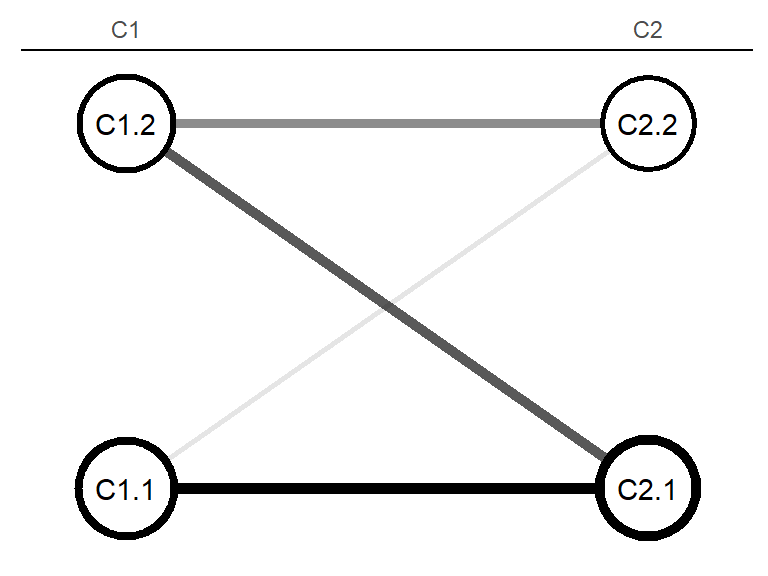
\includegraphics{S23_files/figure-latex/plotlta_2-1} \end{center}

\hypertarget{c.-adding-control-variables-optional}{%
\subsection{2c. Adding control variables (optional)}\label{c.-adding-control-variables-optional}}

If there is time, you can conduct additional analyses, including gender as a control variable.

Click to show answers

You could include gender as a control variable on the observed variables, by adding it to the \texttt{usevariables}, and including the following lines:

\texttt{u11-u15\ ON\ gender;}
\texttt{u21-u25\ ON\ gender;}

Alternatively, you could regress class membership on gender, to see whether men are more likely to be in a particular class than women, or vice versa. This is only allowed when you're NOT using probability parametrization. So, you would have to remove this line:

\texttt{PARAMETERIZATION\ =\ PROBABILITY;}

And add this line:

\texttt{c1\ c2\ ON\ gender;}

\hypertarget{d.-extend-the-model-to-a-mover-stayer-model-optional}{%
\subsection{2d. Extend the model to a mover-stayer model (optional)}\label{d.-extend-the-model-to-a-mover-stayer-model-optional}}

\href{https://www.statmodel.com/download/LTA\%20with\%20Movers-Stayers.pdf}{This Mplus FAQ} explains how to extend the model to a mover-stayer model. At this point, we have to forget about the function \texttt{createMixtures}: It is not suited to estimate the mover-stayer model; it can only estimate simple latent class (growth) models for a varying number of classes. However, we can use this as an opportunity to look at another function in the \texttt{MplusAutomation} package: \texttt{mplusModeler}. This function creates and runs the Mplus syntax in one step:

First, specify the Mplus model. Every argument of the function \texttt{mplusObject} corresponds to a section of an Mplus input file:

\begin{Shaded}
\begin{Highlighting}[]
\NormalTok{mover\_stayer\_model }\OtherTok{\textless{}{-}} \FunctionTok{mplusObject}\NormalTok{(}
  \AttributeTok{VARIABLE =} \StringTok{"CATEGORICAL = u11{-}u15 u21{-}u25;}
\StringTok{              CLASSES = move(2) c1(2) c2(2);"}\NormalTok{,}
  \AttributeTok{ANALYSIS =} \StringTok{"TYPE = mixture;}
\StringTok{              PROCESSORS IS 2;}
\StringTok{              LRTSTARTS (0 0 40 20);}
\StringTok{              PARAMETERIZATION = PROBABILITY;"}\NormalTok{,}
  \AttributeTok{MODEL =} \StringTok{"\%OVERALL\%}
\StringTok{           c1 ON move;}
\StringTok{           MODEL move:}
\StringTok{           \%move\#1\% ! Movers}
\StringTok{           c2 on c1;}
\StringTok{           \%move\#2\% ! Stayers}
\StringTok{           c2\#1 ON c1\#1@1;}
\StringTok{           c2\#1 ON c1\#2@0; }
\StringTok{           MODEL c1:}
\StringTok{           \%c1\#1\%}
\StringTok{           [u11$1] (a1);}
\StringTok{           [u12$1] (b1);}
\StringTok{           [u13$1] (c1);}
\StringTok{           [u14$1] (d1);}
\StringTok{           [u15$1] (e1);}
\StringTok{           \%c1\#2\%}
\StringTok{           [u11$1] (a2);}
\StringTok{           [u12$1] (b2);}
\StringTok{           [u13$1] (c2);}
\StringTok{           [u14$1] (d2);}
\StringTok{           [u15$1] (e2);}
\StringTok{           MODEL c2:}
\StringTok{           \%c2\#1\%}
\StringTok{           [u21$1] (a1);}
\StringTok{           [u22$1] (b1);}
\StringTok{           [u23$1] (c1);}
\StringTok{           [u24$1] (d1);}
\StringTok{           [u25$1] (e1);}
\StringTok{           \%c2\#2\%}
\StringTok{           [u21$1] (a2);}
\StringTok{           [u22$1] (b2);}
\StringTok{           [u23$1] (c2);}
\StringTok{           [u24$1] (d2);}
\StringTok{           [u25$1] (e2);"}\NormalTok{,}
  \AttributeTok{OUTPUT =} \StringTok{"tech15;"}\NormalTok{,}
  \AttributeTok{rdata =}\NormalTok{ data,}
  \AttributeTok{usevariables =} \FunctionTok{names}\NormalTok{(data)[}\SpecialCharTok{{-}}\DecValTok{11}\NormalTok{])}
\end{Highlighting}
\end{Shaded}

Next, run the model we created above. You specify an input file, which will be created, and the argument \texttt{run\ =\ 1L} means you want to run the model. Set it to \texttt{run\ =\ 0L} (the default) to create syntax without running it.

\begin{Shaded}
\begin{Highlighting}[]
\NormalTok{result }\OtherTok{\textless{}{-}} \FunctionTok{mplusModeler}\NormalTok{(}\AttributeTok{object =}\NormalTok{ mover\_stayer\_model,}
                       \AttributeTok{modelout =} \StringTok{"mover\_stayer.inp"}\NormalTok{,}
                       \AttributeTok{run =}\NormalTok{ 1L)}
\end{Highlighting}
\end{Shaded}

Look in the output for the information about the response probabilities for the various latent classes. Also, look for the transition table. Which classes are the movers and which are the stayers?

\begin{Shaded}
\begin{Highlighting}[]
\FunctionTok{get\_class\_counts}\NormalTok{(result)}
\end{Highlighting}
\end{Shaded}

\begin{tabular}[t]{l|r|r|r}
\hline
variable & class & count & proportion\\
\hline
MOVE & 1 & 588 & 0.59\\
\hline
MOVE & 2 & 412 & 0.41\\
\hline
C1 & 1 & 554 & 0.55\\
\hline
C1 & 2 & 446 & 0.45\\
\hline
C2 & 1 & 667 & 0.67\\
\hline
C2 & 2 & 333 & 0.33\\
\hline
\end{tabular}

\hypertarget{e.-selecting-the-number-of-classes-optional}{%
\subsection{2e. Selecting the number of classes (optional)}\label{e.-selecting-the-number-of-classes-optional}}

We have not investigated whether 2 classes is the right number for this dataset. Investigate how many classes at each timepoint you would choose.

Think about:

\begin{itemize}
\tightlist
\item
  Whether you think there should be an equal number of classes at both timepoints (this is mostly a theoretical decision).
\item
  How to build the model. Should you start by comparing unconstrained or constrained models?
\item
  How to decide what solution you prefer.
\end{itemize}

\end{document}
